%Paqueting
\documentclass[11pt, letterpaper, english]{article}
\usepackage[english]{babel}
\usepackage[utf8]{inputenc}
\usepackage[letterpaper, margin=2cm]{geometry}
\usepackage{graphicx}
\usepackage[rightcaption]{sidecap}
\usepackage{float}
\usepackage{array}
\usepackage{amsmath, amsthm, amssymb}
\DeclareUnicodeCharacter{2212}{-}
\usepackage{wrapfig}
\usepackage{enumerate} 
\usepackage{xcolor}
\usepackage[hidelinks]{hyperref} 
\usepackage{latexsym}
\usepackage{hyperref}
\graphicspath{{images/}} 
\hypersetup{
    colorlinks=true,
    linkcolor=black,
    filecolor=blue,      
    urlcolor=blue,
    citecolor=black,
    pdftitle={Math Modelling Manual},
    pdfpagemode=FullScreen,
    }
\usepackage{titlesec}


\setcounter{secnumdepth}{4}

\titleformat{\paragraph}
{\normalfont\normalsize\bfseries}{\theparagraph}{1em}{}
\titlespacing*{\paragraph}
{0pt}{3.25ex plus 1ex minus .2ex}{1.5ex plus .2ex}



%Dates
\title{Math Modelling manual}
\author{iGEM UAM \&  iGEM Tec-Chihuahua \& }

\begin{document}

\begin{titlepage}
   \begin{center}
       \vspace*{1cm}

   {\Huge \textbf{Project Modelling Manual for future iGEM teams}}

       \vspace{0.5cm}
        A look at mathematical/computer modelling in synthetic biology
            
       \vspace{1.5 cm}

\centering\begin{tabular}{>{\centering\arraybackslash} c c c}
iGEM UAM &  & iGEM Tec-Chihuahua \\
igem.uam@gmail.com &  & igemtecchihuahua@gmail.com\\
Universidad Autónoma Metropolitana &  & Instituto Tecnológico y de Estudios\\
 &  & Superiores de Monterrey, Campus Chihuahua\\
 &  & \\
 \end{tabular}
 \centering\begin{tabular}{>{\centering\arraybackslash} c}
 USP-EEL-Brazil \\
symb-lab@usp.br \\
Universidade de São Paulo \\
Escola de Engenharia de Lorena \\
\end{tabular}




  \vspace{1.0cm}
        

\includegraphics[width=12cm]{Logos-Chih-UAM-USP.png}

       \vfill
       \vspace{0.1cm}
       Brazil, Mexico\\
       July 2022
            
   \end{center}
\end{titlepage}


\title{Project Modelling Manual for future iGEM teams}



\nocite{*}

\newpage

\tableofcontents

\newpage 

\section{Introduction}

\par{Mathematical and computational modelling constitutes one of the fundamental pillars of contemporary science. Thanks to it, researchers can successfully predict the behaviour of many systems like the weather, oil wells, cells, and aquifers to the interaction of galaxies. There are multiple ways to model reality. We can use algebra, geometry, or many other mathematical tools. Nevertheless, most of them were done by using differential equations \cite{castillo_2012}.}

\par{Differential equations are used because they capture the dynamic nature of our world. They show how something changes depending on something else (for example, a bucket kept under a running tap is getting filled with water after a certain time\footnote{In this case we will measure the quantity of water in the bucket (our dependent variable) In dependence of the time (our independent variable)}). When only the change of one variable is measured, the equations are called Ordinary Differential Equations (ODE).}

\par{Most complete models measure how variables change depending not only on one independent variable (time, for example) but also on other independent variables (temperature, pressure, and others), this class of equations is called Partial Differential Equations (PDE).}

\par{A mathematical model doesn't need a spotlight for its structural complexity or magnificent theoretical formulation. It can be limited to being an acceptable approximation of reality. A simple model could be functional if it incorporates scientific knowledge, including the general laws of nature, and technological understanding, such as experimental measurements. All utilitarian models, whether explicate or not, are predictive. They allow us to make quantitative predictions, whether deterministic or probabilistic, which can be used either to test and refine the model and for its use in practice.}

\par{Maths Modelling shows the applicability of all kinds of mathematical ideas to 'real-world' problems. Some of these arise in attempts to explain natural phenomena, for example, models for water waves. Other applications are there in the industry, which is a source of many fascinating and non-standard mathematical problems. The industrial processes are not defined in detail. The critical conditions make it expensive and difficult to do detailed experimental investigations. Although, Engineers and other professionals design processes that work fine and be efficient. And if it is not broken, don't fix it: so where does mathematics appear? Some important uses are in quality control and cost control for existing processes, and simulation and design of new ones. We may want to understand why a certain type of defect occurs; what is the 'rate-limiting' part of a process; how to improve efficiency, however marginally; whether a novel idea is likely to work at all, and if so, how to control it \cite{Howison_2008}.}

\par{This manual is based on the work of the Imperial College London iGEM team of 2020, on his guide: \href{https://static.igem.org/mediawiki/2020/9/96/T--Imperial_College--introtomodelling.pdf}{"Introduction to Mathematical Modelling in Synthetic Biology: Version 1"}. Just as our predecessors did, we extend the invitation to any iGEM team to translate or get better our work with absolute freedom. The source LaTeX file can be found on our wiki page and \href{https://github.com/Rexmali/iGEM-UAM2022}{here}.}

\par{The objective of this manual is to extend the excellent guide of \cite{igem_2020} with a practical approach. Due to this objective, we want to present the theoretical bases of Mathematical modelling and its computational implementation.}

\newpage

\section{Justification}

\par{When we started the development of our projects, we were very excited to be able to contribute to our communities through synthetic biology. We  were inspired by the excellent work teams had done in past editions. This led us to seek that each of the areas which we developed in our projects was outstanding. However, at the beginning of our project, one of the first challenges we encountered was starting to model, we felt that we did not know where to start, and when talking with other iGEM teams, we realised that we shared the same thought. In addition, we noticed that the modelling area of the project represents a challenge since, for many teams, the competition is their first approach to modelling biological systems.} 

\par In most college courses, even those focused on biotechnology, the bioinformatics subjects are not enough to teach the mathematical modelling necessary for the competition. Programming classes in engineering and computer courses don't teach about protein modelling. So, since college doesn't prepare us for this, we need something to prepare us for it.

\par{The modelling of a project is a fundamental part of the design of any work. That dwells in a complex system description through mathematical formulas, computational simulations, molecular dynamics, and others. The modelling of the project allows for behaviour predicting of a system before its construction to identify problems and avoid unnecessary spending of time and money.}

\par {Of course, student autonomy in the learning process is meaningful, but the 'learning to learn' idea that happens in modelling is somewhat outdated. Divers teams leave incredible legacies in the bioinformatics area, but there is a lack of content to help them learn, as this process can be exhausting. If modelling is a tool that, as said, helps to save time in the laboratory, why not save time developing it? Certainly, a person responsible for modelling will have to use his thoughts to interpret results and build systems, but there is a lack of tutorials on how to use the software and even a guide to choosing the best one.}

\par{There were months of research, mentoring, self-learning and supporting each other between teams to develop acceptable models. During the development of the competition, we learned a lot. However, au courant that if knowledge is not shared, it is useless. So, we decided to find a way for the learning we had acquired about project modelling to transcend, and that is how the idea of writing this manual was born.} 

\par{Likewise, we saw the manual as a way to repay all the support we have received for our project's development. Throughout our history at iGEM, we have received help from many people such as mentors, instructors and other teams that have supported us in our project, especially in modelling. Without them, the development of our projects would not have been possible. Just as they shared their knowledge and experience with us, we want to share it with other iGEM teams worldwide, but mainly with Latin American teams, which is why it is available in English, Spanish and Portuguese. Additionally, it is a way to contribute to the development of scientific knowledge in our native languages. In the same way, it can also be practical for people outside of iGEM. Nevertheless, every iGEM team could translate this manual so that anyone has access to this information.} 

\par{We are aware that diversity enriches us and helps us go further. This is why, as American non-English speakers teams, iGEM Tec Chihuahua, iGEM UAM of México and USP-EEL from Brazil, coalesce to work on this manual. We understand the necessity of other iGEM teams to get scientific knowledge in their corresponding native languages. Being part of the few LATAM teams that will participate this year in the competition, we want to afford something valuable for iGEM Community.

We are grateful that the Imperial College London team allowed us to base ourselves on their manual made in 2020.
Thus, with the sum of the knowledge of each team, and the knowledge that we develop together by working hand in hand, we seek to generate different approaches and perspectives on project modelling.}

\par{We hope that this manual will serve as a first-step guide for future equipment.}



\section{Objectives}

\begin{enumerate}
    \item Describe, explain and facilitate the principles of a mathematical model to the iGEM teams of Latin America. 
        \begin{enumerate}
            \item  Describe what a mathematical model is and how it is used to simplify.
        \end{enumerate}
    \item Explain the types of mathematical models that  can be used and the advantages they present when modelling different biological phenomena.
    \item Describe the bioinformatic tools available to implement in an iGEM project
    \item Understand how it is possible to perform computational simulations of mathematical models with a biological approach.
    \item Exemplify models of biological systems that can serve as a basis for new work.
    
\end{enumerate}

\newpage



\newpage

%%%%% Mathematical tools
\section{Mathematical tools}

\subsection{Differential Equations}

\par{A differential equation (DE) is a relationship between a function of time and its derivatives. Differential equations come in many forms and are an essential concept for much of maths and science. The equations \ref{eq1} and \ref{eq2} are both examples of differential equations. In modelling the dynamics of a system where the variables vary with time, we can form DEs to model this variation. Cell processes such as transcription and translation take time, so we have to describe the variation of mRNA and protein concentrations using differential equations and then attempt to solve those equations.}

\begin{equation}
    \frac{d y}{d t}=3 y^2 \sin{\left( x+t  \right)}
    \label{eq1}
\end{equation}

\begin{equation}
    \frac{d^3 y}{{d t}^3}=\exp{-y} + t + \frac{d^2 y}{{d t}^2}
    \label{eq2}
\end{equation}

\subsubsection{Characterisation}
\par{The differential equations' properties and their solutions can be analysed based on their characterisation. A basic understanding of these categories is utile.}

    \paragraph{The order of a differential equation}
    
    \par{The order of a differential equation is the order of the highest derivative of the function y that appears in the equation. Thus Equation \ref{eq1} is a first-order differential equation and Equation \ref{eq2} is a third-order differential equation}
    
    \paragraph{Number of independent variables}
    
    \par{\textit{Ordinary differential} equations (ODEs) have a dependent variable (and its derivatives) which only depends on one independent variable. On the other hand, \textit{partial differential} equations (PDEs) have a dependent variable depending on two or more independent variables. PDEs are a lot more complex to solve.}
    
    \paragraph{Homogeneity of differential equation}
    
    \par{The Equation \ref{eqhomo} is called the homogeneous first-order linear differential equation, and Equation \ref{eqhomo2} is called the non-homogeneous first-order linear differential equation for b(t) not identically zero. Homogeneous means every term contains the dependent variable or its derivatives, while inhomogeneous implies there is at least one term which does not.}
    
    \begin{equation}
        \frac{d y}{d t}+a(t) y =0
        \label{eqhomo}
    \end{equation}
    
    \begin{equation}
        \frac{d y}{d t}+a(t) y =b(t)
        \label{eqhomo2}
    \end{equation}

    
    \paragraph{Linearity of differential equation}
    
    \par{Linear implies every term is of the form coefficient × derivative, such that the dependent variable and its derivatives are never in any function. We call linear equation because the dependent variable y appears by itself, that is, no terms such as $e^{-y}$, $y^3$ or $\sin{(y)}$ etc. appear in the equation. For example $\frac{dy}{dt} = y^2 + \sin{t}$ and $\frac{dy}{dt} = \cos{(y)} + t$ are both nonlinear equations because of the $y^2$ and $\cos{(y)}$ terms respectively. \cite{braun_1993}}

    \paragraph{Systems of differential equations }
    
    \par{Coupled implies there are two or more DEs in which they share two or more dependent variables. In this way, the variation of the dependent variable of one DE depends on the variety of the dependent variable of another DE. Systems of DEs have the form: }

    \begin{equation}
    \begin{split}
    \frac{d x_1}{dt}=f_1(t,x_1,x_2,...,x_n)\\
    \frac{d x_2}{dt}=f_2(t,x_1,x_2,...,x_n)\\
    . \\
    . \\
    . \\ 
    \frac{d x_n}{dt}=f_n(t,x_1,x_2,...,x_n)
    \end{split}
    \end{equation}

    \subsubsection{Solutions}
    
    \par{The DE solutions are functions which satisfy the equation such that no derivatives are present in the solution. Frequently, DEs can’t be solved analytically (a general algebraic solution). This is because integration is sometimes impossible for more complex equations (such as the Hill equation, in general). However, they can be solved numerically using iterative computational methods. There are many different methods for different situations, but programs like MATLAB or packages like Scipy in Python have functions which do the hard work.}

    \subsection{Mass Action Kinetics (MAK)}
    
    \par{Mass action kinetics is a framework to analyse chemical reactions based on the assumption that the rate of those reactions can be modelled by the concentration of the reactants. There is also a coefficient of proportionality to be found empirically. Once these coefficients are known, the rate equation (a DE) can be solved to provide a model to describe how concentrations vary with time.}
    \par{The following sections describe different cases where this law is used.}
    
    \subsubsection{A Simple Reaction}

    \par{Consider the following reaction}

    \begin{equation}
        A \rightarrow C.
    \end{equation}

    \par{For every one A that reacts, one C is outputted as the product. That is, for every reaction, one C is created and one A is used up. Given C doesn’t react, the rates won’t be dependent on C. In this equation, we would model the rates as its shown in Equation \ref{Eq7} and Equation \ref{Eq8}.}

    \begin{equation}
        \frac{d [A]}{d t}=-k[A]
        \label{Eq7}
    \end{equation}

    \begin{equation}
        \frac{d [C]}{d t}=k[A]
        \label{Eq8}
    \end{equation}
    
    \par{Where k is a constant describing the relative velocity of the reaction. As A decreases, the concentration decreases. As C is produced, the concentration increases. Since the rate of C outcome is equivalent to the rate of A reduction, the equations are very similar.}

    \subsubsection{Reverse Reaction}

    \par{Suppose we introduce the reverse reaction, so C can react and go back to A:}

    \begin{equation}
        A \rightleftharpoons C.
    \end{equation}

    \par{This would mean we effectively have two reactions, A to C and C to A. The new rates are the sum of these two ODEs. Therefore, in total, we have the following equations [\ref{Eq10}, \ref{Eq11}].}

    \begin{equation}
        \frac{d [A]}{d t}=-k_1[A]+k_2[C]
         \label{Eq10}
    \end{equation}


    \begin{equation}
        \frac{d [C]}{d t}=k_1[A]-k_2[C]
         \label{Eq11}
    \end{equation}

    \subsubsection{Two Reactants}

    \par{Let’s further the complexity, and add an additional reactant:}

    \begin{equation}
        A+B \rightleftharpoons C.
        \label{eq12}
    \end{equation}

    \par{Intuitively, we see that an A and a B must react to make a C. This means that if there is no A, no reaction will occur. Which implies rate is dependent on the concentration of A and B in one combined term. Likewise, the reverse reaction only depends on C and produces an A and a B. Therefore, we have three rates here:}

    \begin{equation}
        \frac{d [A]}{d t}=-k_1[A][B]+k_2[C]
        \label{eq13}
    \end{equation}

    \begin{equation}
        \frac{d [B]}{d t}=-k_1[A][B]+k_2[C]
        \label{eq14}
    \end{equation}

    \begin{equation}
        \frac{d [C]}{d t}=k_1[A][B]-k_2[C]
    \end{equation}

    \par{Note that the rate of change of A and B are equal because the reaction will occur without any reactant.} 

    \subsubsection{Reaction Coefficients}

    \par{Consider the reaction}

    \begin{equation}
        2A \rightleftharpoons C.
        \label{eq16}
    \end{equation}

    \par{Referencing section C, we observe that the rates will be given as is shown in Equation \ref{eq17} and in Equation \ref{eq18}}

    \begin{equation}
        \frac{d [A]}{d t}=-k_1[A][A]+k_2[C]=-k_1{[A]}^2+k_2[C]
        \label{eq17}
    \end{equation}

    \begin{equation}
        \frac{d [C]}{d t}=k_1[A]^2-k_2[C]
        \label{eq18}
    \end{equation}

    \par{So the coefficient in the reaction equation will be the power in the rate equation. We can generalise the equations (\ref{eq12}), (\ref{eq13}) and (\ref{eq16}) as:}

    \begin{equation}
        nA+mB \rightleftharpoons C.
    \end{equation}

    \par{With the change of rate:}

    \begin{equation}
        \frac{d [A]}{d t}=\frac{d [B]}{d t}=-k_1{[A]}^n[B]^m+k_2[C]
    \end{equation}

    \par{and}

    \begin{equation}
        \frac{d [C]}{d t}=k_1[A]^n[B]^m-k_2[C]
    \end{equation}


    \subsubsection{Degradation}

    \par{In some instances, a molecule may degrade to some other species which isn’t relevant to the system in question and cannot revert to the original molecule. We write this as:}
    
    \begin{equation}
        A \longrightarrow  \varnothing
    \end{equation}
    \par{This is modelled just as in part A, but there is no product. Instead, we ignore it since we only care about certain species within a system. The rate coefficient for degradation is typically given as $\delta$, giving the rate equation [\ref{eq23}].}
    
    \begin{equation}
        \frac{d [A]}{d t}=-\delta[A]
        \label{eq23}
    \end{equation}
    
    \par{This is modelled just as in part A, but there is no product. Instead, we ignore it, since we only care about certain species within a system. The rate coefficient for degradation is typically given as $\delta$, giving the rate equation}
    
    \subsubsection{Example}
    
    \par{Given the chemical equation for the production of hydrogen chloride from hydrogen and chloride find the correct rate equation for hydrogen chloride (The forward reaction rate is equal to $K_F$ and the backward reaction rate is equal to $K_B$): }
    
    \begin{equation}
        H_2+{Cl}_2 \rightleftharpoons 2HCl
    \end{equation}
    
    \vspace{2 cm}
    
    \begin{equation}
        A)\frac{d [HCl]}{d t}=+k_F[H_2][{Cl}_2]-k_B[HCl]^2
    \end{equation}

    \begin{equation}
        B)\frac{d [HCl]}{d t}=+k_F[H_2][{Cl}_2]-k_B[HCl]
    \end{equation}

    \begin{equation}
        C)\frac{d [HCl]}{d t}=+k_F{[H]}^2{[Cl]}^2-k_B[HCl]^2
    \end{equation}
    
    
\subsection{Hill Equation}
    
\par{In any reaction where two species bind together, they may unbind and return to their constituent parts. This is the same form as in section 2.2.3, but where the larger species may have multiple binding sites, such that we have a reaction equation of the following form:}
    
\begin{equation}
    A+mB \rightleftharpoons C.
\end{equation}
   
\par{Where A is the larger species, B is the smaller species, C is the complex formed from the binding and n is the number of binding sites on A. For example, the binding of a ligand to a macromolecule, a transcription factor to a promoter, or a substrate to an enzyme. Using MAK, we can derive an equation called the Hill Equation from the rate equation, based on a few assumptions. While it has limitations in its accuracy, the Hill Equation is a good starting point when the dynamics of the binding are unknown.}
    
    \subsubsection{Derivation}
    
    \par{We define the forward reaction constant $k_a$ for association and the reverse reaction constant $k_d$ for dissociation. Considering the ODE for the complex using MAK, we therefore have}
    
    \begin{equation}
        \frac{d [C]}{d t}=k_A{[A]}[B]^m+k_d[C]
    \end{equation}
    
    \par{If $[C]$ is initially zero, the concentrations will shift until the forward reaction rate is equal to the reverse reaction rate, such that the concentrations no longer vary with time. We call this point equilibrium. This means at equilibrium, the concentration of the complex won’t vary with time. Therefore, we equate this equation to zero:}
    
    \begin{equation}
        \frac{d [C]}{d t}=k_A{[A]}[B]^m+k_d[C]=0
    \end{equation}
    
    \par{Rearranging, we define the apparent dissociation constant, $K_d$, as the ratio of the dissociation rate constant and the association rate constant.}
    
    \begin{equation}
        K_d = \frac{k_d}{k_a}=\frac{[A]{[B]}^m}{[C]}
        \label{eq31}
    \end{equation}
    
    \par{We can then calculate the proportion of bound A molecules to the proportion of total A molecules (bound and unbound), which we call $\theta$:}
    
    \begin{equation}
        \theta= \frac{Bound A molecules}{Total A molecules}=\frac{[C]}{[A]+[C]}
    \end{equation}
    
    \par{Remembering that A is the larger species.}
    
    \par{Using equation (\ref{eq31}), we can substitute [C] = [A][B]n $K_d$ and rearrange to get the equation.}


    
    \par{This is the proportion of the Complex molecule (bound A) to the total number of A molecules in terms of their concentrations. It is also possible to find the proportion of unbound A molecules, simply by calculating $(1-\theta)$.}
    
    \begin{equation}
        \theta = \frac{ \frac{[A]{[B]}^m}{K_d} }{ [A] + \frac{[A]{[B]}^m}{K_d} }= \frac{[A]{[B]}^m}{[A] K_d + [A] {[B]}^m} = \frac{{[B]}^m}{ K_d + {[B]}^m}
    \end{equation}
    
    \subsubsection{Limitations}
    
    \paragraph{Assumption}
    
    \par{Assumes all B's bind to A simultaneously, as opposed to in succession over some time.}
    
    \par{Does not account for the interaction between successive B's and their cooperativity (this model assumes very positive cooperativity).}
    
    \par{Does not consider partial binding (i.e. not all binding sites filled), and the functionality of this partially bound complex.}
    
    
\newpage
% !!! COMENTARIO aquí eran los tipos de modelos matemáticos? optimisation es un modelo?
\section{Models to use and characteristics} 
\par{A mathematical model is a formal expression (in language mathematical) of the relationships between the components of a model. Building a model of this type implies selecting and quantifying the components variables and relationships present in the system to represent it with the required level of detail. It can be something as simple as substituting the variables of an equation with its real values or it can be a complex set of interrelated equations whose variables are modified over time and across space. \cite{Modelos}}
\par{The mathematical language allows describing and modelling systems in a parsimonious way, objective and unambiguous; to the point that today mathematical models are considered theories about the systems being modelled. The symbolic language provided by mathematics allows the expression of highly complex ideas.} \cite{Modelos}
\par{A distinction must be made between this conception of a model, as a representation of a theory by means of an equation more or less simple, and the idea of a model as a group of a set of equations (which respond to different theories) interconnected in a way that represents the different transfers between the components of the modelled system. \cite{Modelos}}
\par{Desirable features of mathematical models are:}
\subsection{Characteristics}
\begin{itemize}
    \item Parsimony, a model is not necessarily better for having many parameters. simplicity is always desirable.
    \item Modesty, they should try to achieve only attainable goals. A model, like a map, does not it should aspire to imitate reality but only to highlight those aspects of interest for its application.
    \item Accuracy, the model must reproduce as far as possible the operation of the system and generate values for the output and state variables similar to those observed in reality.
    \item Verifiability, the model's results must be able to be compared with real data and determine from this mode the degree of accuracy of the model.
    \item  On the other hand, it is not enough that they work well, they must work well for the right reasons.
    \end{itemize}.

    \begin{enumerate}
        \item Determinism
    \par{To say that a system is deterministic means that each state is completely determined by the previous state. 
    For example in the food chain model, just as in all the other models we have studied, there are no unmodelled outside influences or chance events. If we allow outside chance events, it is easy to produce an irregular time series by, say, flipping a coin, but there’s nothing like this in the food chain model or the discrete logistic model. The system is deterministically producing its own irregular behaviour without any randomness. \cite{garfinkel_shevtsov_guo_2017}.}

    \item{Boundedness}

    \par{It means that the system does not go off to infinity. As the figure below illustrates, it stays within an assured region of state space. In other words, we could draw a box in a stationary space, and the system would stay within that box. And in the discrete logistic model, as long as our initial condition is within the interval (0, 1), the result will always be in that interval; the state point will not escape to higher values \cite{garfinkel_shevtsov_guo_2017}.}
    
    \begin{figure}[ht]
	    \centering
		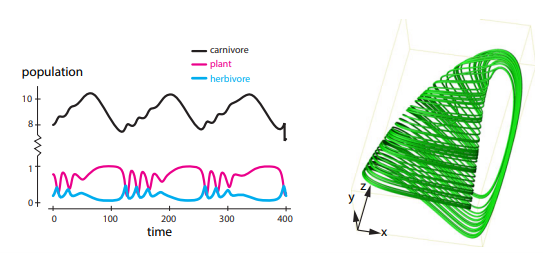
\includegraphics[width=0.7 \textwidth]{Chaos.png}
		\label{Imagen_1}
		\caption{Left: a simulation of the three-species food chain model described in the text with a1 = 5, b1 = 3, a2 = 0.1, b2 = 2, d1 = 0.4, and d2 = 0.01. Right: a typical trajectory of the three-species model, Obtained from: \cite{garfinkel_shevtsov_guo_2017}}
	\end{figure}

	\item{Irregularity}
	
	\par{Chaotic behaviour is irregular or aperiodic. Aperiodic behaviour never exactly repeats. If a trajectory ever exactly repeated, that is, returned to the very same mathematical state point, it would have to be periodic because determinism would require that it return again and again. All closed orbits are periodic trajectories. Hence, limit cycle attractors are closed periodic orbits. Systems with point or limit cycle attractors have initial transients but then settle down into repetitive behaviour. Chaotic behaviour, on the other hand, starts out irregular and remains irregular. In some systems, it may look like the behaviour repeats and it can come very close to previous state values, but it never exactly repeats \cite{garfinkel_shevtsov_guo_2017}.}

 
	 \begin{figure}[ht]
	    \centering

		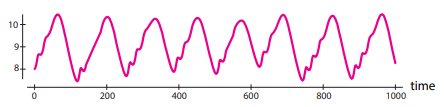
\includegraphics[width=0.7 \textwidth]{Irregularity.png}
		\label{Imagen_2}
		\caption{Time series of the carnivore population from a typical simulation of the three species food chain model., (Obtained from  \cite{garfinkel_shevtsov_guo_2017})}
	\end{figure}

 
    \par{At first glance, it seems the populations oscillate, albeit in a complex way. However, a closer look reveals differences. The second large oscillation contains one bump before the peak, while the third oscillation has at least two. Moreover, each peak has a somewhat different shape. This is aperiodicity. Despite a general qualitative similarity, the behaviour of the system never repeats and never approaches repetition. A similar statement is true about the output of the discrete-time logistic model. It may look as though some shapes repeat themselves, but if we look closely, we see that the sequence, in fact, never repeats.  \cite{garfinkel_shevtsov_guo_2017}}
    
    \item{Sensitive Dependence on Initial conditions}
    \par{The most intriguing and famous characteristic of chaos is the sensitive dependence on initial conditions. This term refers to the fact that in a chaotic system, two-time series that start very close together will eventually diverge to the point where their behaviour is completely uncorrelated. In general, for multivariable systems, in both discrete and continuous time, sensitive dependence means exponential divergence of nearby trajectories: there is a number $\lambda$ (greek letter lambda), called the Lyapunov characteristic exponent, such that:} 
    
    \begin{equation*}
    d ( M_{t} − N_{t} ) = e^{ \lambda  t}  d ( M_{0} − N_{0} )  
    \end{equation*}

    \vspace{0.5 cm}

    \item{Unpredictability}
    
    \par{Perhaps, you already heard about Edward Lorenz, the meteorologist and mathematician who helped discover chaos. He gave a meeting called “Predictability: does the flap of a butterfly’s wings in Brazil set off a tornado in Texas?” He posed a question: Consider two planets that are absolutely identical, down to the clothes you are wearing today, every tree, every detail, except that in world A there is one more butterfly in Brazil. What will happen to the weather systems of the two planets? Maybe you thought  there will be no difference from such an infinitesimal change, but common sense is wrong. In fact, after not much time, the weather systems will diverge completely, so there is, say, a tornado in Texas in world A but not in world B! 
    Sensitive dependence on initial conditions helps explain a fundamental property of chaotic behaviour, it is unpredictability. \cite{garfinkel_shevtsov_guo_2017}}
    \end{enumerate}
\subsection{Models to use}



\subsubsection{Deterministic}

\par{The deterministic model is a mathematical prototype \cite{Witenberg_1995}, where the same inputs will invariably produce the same outputs, regardless of consideration of the existence of chance or uncertainty. Knowing with certainty the values of the variables, then, it will be assumed that we have all the information necessary for the evaluation of a project\cite{ramos_2019}.}

 \subsubsection{Stochastic model}

\par{Stochastic models represent the randomness and provide estimates of the media parameters that determine fluid flow, pollutant transport, and heat–mass transfer in natural porous media. This model was developed by Ball in 1986. Ball discussed that the distribution of an infectious period is allowed to be described by its Laplace transform. Stochastic models are built around random graphs. The stochastic process is the study of how a random variable evolves. An unknown variable before a certain time t is called a random variable. If is known the state of the random variable before a period it is called a discrete stochastic process. The Markov chain process is the best example of a stochastic model where the probability distribution of time t + 1 depends on the state at time t and does not depend on the states before time t \cite{stochastic_model_overview_sciencedirect} \cite{statistical_models_2003}.}
    %% añadir imagen cadena markov

% !!! COMENTARIO aquí no tenemos ninguna cita?
\subsubsection{Monte Carlo Method}

    \par{It is a mathematical technique used to estimate the possible outcomes of an uncertain event. The Monte Carlo method was invented by John von Neumann and Stanislaw Ulam during World War II to improve decision-making under conditions of uncertainty. Its name comes from a well-known casino in Monaco, as the element of chance is at the core of the modelling approach, similar to a roulette game. Monte Carlo simulations have evaluated the impact of risk in many real-life scenarios, including artificial intelligence, stock prices, sales forecasting, project management, and pricing. They also provide several benefits for predictive models with fixed inputs, such as performing sensitivity analysis or calculating input correlation. Sensitivity analysis allows decision-makers to see the impact of individual inputs on a given outcome, and correlation allows them to understand relationships between input variables\cite{garfinkel_shevtsov_guo_2017}.}
  

\subsubsection{Optimisation}
    \par{Many efforts have been made to describe complex human and social situations. To be written in a mathematical expression containing one or more variables, its values must be determined. The question that is formulated, in general terms, is for what values these variables should have a mathematical expression which has the greatest possible numerical value (maximisation) or the smallest possible numerical value (minimisation). This general process of maximisation or minimisation is called optimisation. Optimisation is used to find the answer that provides the best result, to achieve the highest profits, production or happiness, or to get the least cost, waste or discomfort. Frequently, these problems involve the most efficient use of resources, such as money, time, machinery, personnel, inventory and others. Optimisation problems usually are classified as linear and non-linear, depending on whether the relationships of the problem respect the variables.\cite{Arsham_1996}}

    
    % !!! COMENTARIO aquí no tenemos ninguna cita?
  %%Complex       
    \subsubsection{Complex}
    \par{A complex model constitutes the mathematical description of a complex object. Lies on interrelated component elements, that can also be embodied by their own interdependent elements. Also, complex objects and their elements have functions that can be broken down in time, because, in the general case it is required to make decisions related to the system in different periods. A system and its elements act as interferences of the surrounding world. The more complete will be the organisation of the system, the smaller will be the interferences, but the higher the complexity of the conciliation of its operation  \cite{garfinkel_shevtsov_guo_2017}.}
    \par{The difference between  the words complex and complicated are the following:
    \begin{itemize}
        \item Complicated is something consisting of a lot of different parts or details and therefore difficult to understand, but you can solve a 'complicated' problem by analysing separately the different parts.
        \item Complex derived from Latin cum (many) plexus (past participle 'complecti' meaning tighten, embraced. Therefore a complex situation, a complex system or a problem resulting from the union of several parts or elements, became inseparable.
    \end{itemize}}
    
    \subsubsection{Chaotic}
    \par{The concept of chaos is one of the major discoveries of recent times. Chaos is observed every day in metrology, fluid flow (turbulence), cardiology, population biology, the stock market, economic modelling et cetera. Predictions are possible in many systems. For example, eclipses are predicted thousands of years in advance. The motion of a simple pendulum, under suitable assumptions, is governed by a differential equation, predictable and a closed-form solution can be written. However, there are many non-predictable natural phenomena, such as weather predictions, the roll of the dice and so forth. Even though, they obey the same laws of physics. It is believed that predictability can be achieved by having more information and processing it. Some systems are 'chaotic', extremely sensitive to small perturbations and unpredictable in the long run, showing the so-called 'butterfly effect'. \cite{garfinkel_shevtsov_guo_2017}}
    
    
    
     
  
   
    
\newpage

\section{Computational tools in modelling}

\par{In order to build a mathematical model, first, it is necessary to select the structure that we would like the differential equations to have. Next, the partial differential equations will transform into a system that has a finite number of degrees of freedom. This means that the system depends on a definite number of variables and parameters.}


\par{Commonly, a simple equation has only one unknown, and a system of three variables has three unknowns. But in real modelling systems, it is required to transform the differential equations into systems of equations with many unknowns by employing numerical methods  \cite{garfinkel_shevtsov_guo_2017}.}

\par{Mathematical modelling is done before the formulation of any computer idea. We would take the wave equation as an example:}

\begin{equation}
    \frac{\partial^2 y}{{\partial x}^2}=\frac{1}{\nu^2} \frac{\partial^2 y}{{\partial t}^2}
\end{equation}

\par{The wave equation regulates or rules the behaviour of sound. It is possible to solve it by hand if we assume that all space was homogeneous: }

\begin{equation*}
    y= A \cos{ \left( k x - \omega t - \phi \right) }
\end{equation*}

\par{with:}

\begin{equation*}
    \nu = \frac{ \omega }{ k }
\end{equation*}

\par{Thanks to this equation, the theoretical speed of sound was discovered, and its approximation was extremely close to the experimental one. Nonetheless, some mathematical problems can only be solved by a computer, such as sound moving in a heterogeneous medium  \cite{garfinkel_shevtsov_guo_2017}.}

\par{By utilising numerical methods we can find their solutions given by approximations. They imply diverse operations, such as adding, subtracting, dividing, and deriving, among others, which allow reducing the complexity of an equation, but increase the number of solution algorithms  \cite{garfinkel_shevtsov_guo_2017}.}



%PARTE 2.1
    \subsection{Programming languages}
    
    \par{Programming languages are a tool that can be implemented to develop computer programs (software). They can be employed to design and execute instructions to control the behaviour of the physical  (hardware), as well as, logical devices of the computer \cite{monterde_2020}. They are made up of a series of syntactic constituents which provide structure and give meaning to their elements and expressions  \cite{garfinkel_shevtsov_guo_2017}.} 
    
     \par{On the other hand, programming is the process of analysis, design, implementation, testing, and debugging of an algorithm, without these elements, the computer will not be able to perform the task desired by the user  \cite{garfinkel_shevtsov_guo_2017}.} 

    \par{The major function of programming languages is to write programs capable of establishing user-machine communication. In order to do that, programs transform the instructions written to source code,  meaning, instructions written in machine language or binary code (0 and 1). As for compilers, they translate the symbols of a programming language to their equivalent written in machine language. This process is known as compiling (See. Figure. 3). Finally, an executable program is obtained  \cite{garfinkel_shevtsov_guo_2017}.}
   
    %Imagen 1
	\begin{SCfigure}[0.7][ht]
	    \centering
		\caption{What is a compiler?, (Obtained from: \href{https://codeforwin.org/2017/05/compiler-and-its-need.html}{Code Forwin})}
		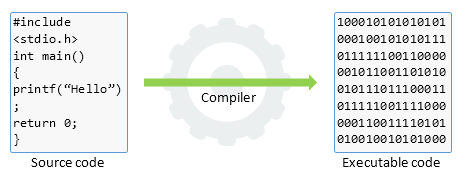
\includegraphics[width=0.7\textwidth]{compiler}
		\label{Fig-Compiler}
	\end{SCfigure}


%Antecedentes
\textbf{Background}

\par{In the mid-19th century, Charles Babbage, a professor of mathematics and inventor at the University of Cambridge, England, was the first to conceive the idea of a programming language. Ada Lovelace is considered the first programmer in history. She wrote the first program for the machine envisaged by Babbage on punched cards by following programming logic. Which is very similar to what we use. Nevertheless, these programs could never run because the machine had not been built  \cite{garfinkel_shevtsov_guo_2017}.} 
\vspace{0.5 cm}
	
	
\par{In 1823, the  British government approved the project to build a different engine designed to perform repeated additions. Babbage abandoned the project to pursue an Analytical Engine. Influenced by the creation of a French cloth manufacturer, Joseph Marie Jacquard, who had developed a machine capable of reading information encoded on punched cards of stiff paper (a sheet made of cardboard that contains information in the form of perforations according to a binary code). Since then, Babbage decided to build a machine that would perform precise calculations using 20 digits. That could be programmed using punch cards  \cite{garfinkel_shevtsov_guo_2017}.} 

%Imagen 2
\begin{SCfigure}[0.5][ht]
	    \centering
		\caption{Punch card, (Obtained from: \href{https://mujeresconciencia.com/2018/06/27/tarjetas-para-programar-el-mundo/}{Women with science})}
		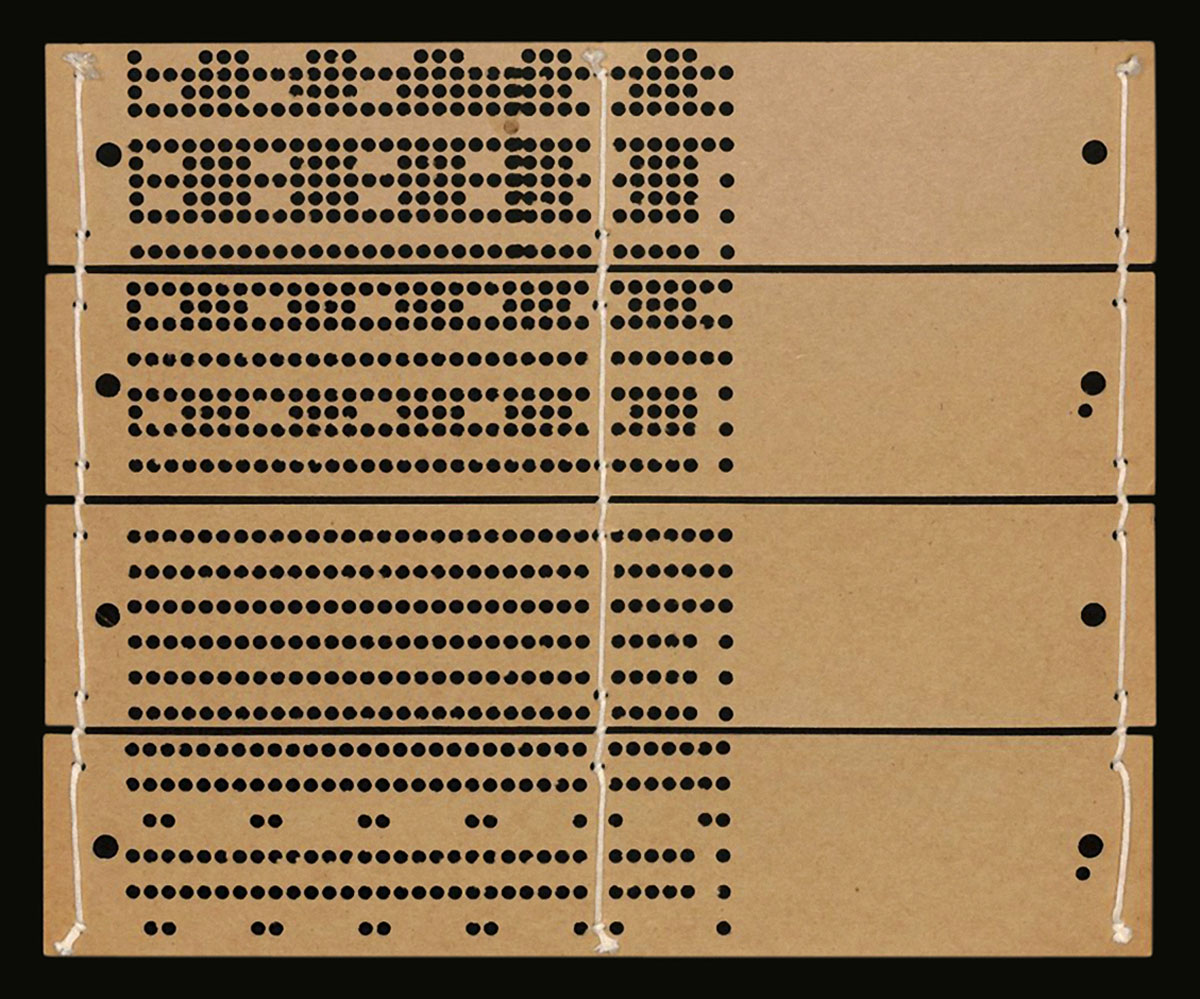
\includegraphics[width=0.5 \textwidth]{Tarjeta.jpg}
		\label{Fig-Perforada}
\end{SCfigure}

\par{Even though, this idea remained only in the project, it was a meaningful contribution to the design and operation of nowadays' computers. Charles Babbage is considered the father of computing. Although the machine was an inspiration, his ideas and design served to build and advance the first modern computers  \cite{garfinkel_shevtsov_guo_2017}.}

\vspace{0.5 cm}

%Clasificación
   \textbf{Clasification}
   \par{Microprogrammable circuits are digital systems, that work with two voltage levels symbolised by zero (0) and one (1). The classification of language types is shown below:}
   
   \begin{itemize}
       \item{Low-level programming language: It provides little or no abstraction of a computer's microprocessor, referring to  binary code. Since it is geared to the hardware, it works as instructions for the processor, and with it is possible to build operating systems and kernels.}
        \item{High-level programming language: It is distinguished by its semantic structure, which allows algorithms to be encoded more naturally.}
   \end{itemize} 
   
  
   %Tabla de ejemplos
    \begin{table}[ht]
        \centering
        \resizebox{4.5 cm}{!} {
        \begin{tabular}{| c | c |}
            \hline
            Low level  & High level \\ \hline
            Assembler   & C++ \\
            LOAD X      & Fortran \\
            ADD Y       & Java \\
            STORE Z     & PHP \\
            -           & Python \\
            -           & Perl \\ \hline
        \end{tabular}}
        \caption{Examples}
   \end{table}
   
   
    %Programming Types
   \textbf{Programming Types}
   \begin{itemize}
       \item{\textbf{Logical programming:} it is characterised by programming with relationships and inference. Here the programmer is responsible for specifying the basic logical relationships.}
       \item{\textbf{Functional programming:} it is characterised by programming with values, functions, and functional forms, which are a relationship between a dependent variable and an explanatory variable. 'A functional program consists of an expression, let us call it E, which is subject to written rules. The reduction consists in replacing some part P of E with another expression P' according to the rules, this process is repeated several times until the expression resulting has no parts that have to be rewritten. The expression obtained from this process, E' is what will be the normal form of E and is the output of the functional program.' -H.P. Barendregt.}
       \item{\textbf{Imperative Programming:} this is characterised by programming with a state and commands that modify it. We have two important parts: imperative, which is an order or command, and procedure, the act, the method of proceeding, or a way of doing something. When imperative programming is combined with other subprograms it is called procedural programming  \cite{garfinkel_shevtsov_guo_2017}.}
      \item{\textbf{Concurrent programming:} is characterised by programming with more than one process. This type of programming is used for compile design, some problems are solved in a natural way using a set of processes that operate at the same time, a sequential solution that builds on specifications and reduces execution time. There is a difference between sequential and concurrent operations. Sequential occur one after another while concurrent is when they occur at the same time  \cite{garfinkel_shevtsov_guo_2017}.} \item{\textbf{Object-oriented Programming:} this kind of programming is characterised by programming with objects, messages, and object hierarchies. Focuses on passive data elements defined by relationships or acts on functions and processes for active elements with their environment  \cite{garfinkel_shevtsov_guo_2017}.} \end{itemize} 
      %Programming languages 
      \textbf{Some programming languages} 
      \begin{itemize} 
      \item{ \textbf{C:} large programs are divided into small programs called functions that are focused on functions and processes that operate with data. It is used in information technology, engineering, management, healthcare, image processing, and game programming.} 
      \item{\textbf{C\#:} is a multi-paradigm programming language with strong programming disciplines. Writing, imperative, declarative, functional, and object-oriented. It is used in information technology, engineering, design, and quality control.} 
      \item{\textbf{C++:} is an object-oriented language, it is a middle-level language, and it is an extension of the C language. It is used in information technology. information, engineering, design, quality control, administration, software, and firmware drivers. } 
      \item{\textbf{Python:} is a programming language that is interpreted, object-oriented, and built on flexible and robust semantics. It is used in Back-end development, information technology, engineering, design, web development, frameworks, advanced content management, scientific and numerical computing, and desktop graphics.} 
      \item{\textbf{Ruby:} is an open-source, object-oriented scripting language that can be used stand-alone or as part of the Ruby on Rails web framework. It is used in the development, software engineering, data science engineering, WebApp development, robotics, networking, system administration, and security.} 
      \item{\textbf{PHP:}  is an open-source scripting language designed to create dynamic web pages that work effectively with databases. It is also used as a general-purpose programming language. It is used for information technology, engineering, design, health care, finance, administration, web application development, and scripting.} 
      \item{\textbf{Java:} is a high-level, user-oriented programming language. objects and general purpose with various features that make it ideal for web-based development. It is used in communication, education, finance, life sciences, retail and utilities, the Internet of Things, the Cloud, video games, and mobile apps.}
      \item{\textbf{JavaScript:} is a client-side programming language that runs inside a client browser and processes commands on a computer instead of a server. It is normally placed in an HTML or ASP file. It is used in Information Technology, Engineering, Design, Marketing, Finance, Healthcare, Front-End Development, and Game Development. Java and JavaScript are not related} 
      \end{itemize} 
   %%%%%%%%%%%%%%%%%%%%%%%%%%%%%%%%

   
\subsection{Computational power and its importance}
    
\par{Supercomputers are massive computing machines used to perform complex calculations in a wide variety of scientific applications. Such applications span a wide range of computationally intensive tasks, including quantum mechanics, weather forecasting, climate research, oil and gas exploration, molecular dynamics, and physical simulations, and require an amount of computing power and resources that go beyond what is available in general for  computer servers or workstations purpose \cite{(R. Gioiosand a 2017)}. These supercomputers are rated according to their performance based on Floating Point Operations Per Second (FLOPS). various features measure mainly indicates the number of operations of this type that the hardware processor can solve in one second by mixing small, large, and even fractional numbers \cite{(McDonell, 2013)}.}

\par{This approach was very expensive and limited the use of supercomputers in a few research centres around the world. To reduce the acquisition and operational costs, researchers started to build supercomputers out of “common-off-the-shelf” (COTS) components, such as those used in general-purpose desktops and laptops. Currently, supercomputers consist of a multitude of compute nodes interconnected through a high-speed network. Each compute node features one or more multicore/multithreaded processor chips, several memory modules, one/two network adapters, and, possibly, some local storage disks. More recently, accelerators, in the form of graphical vector units or field-programmable gate arrays (FPGA), have also made their way to mainstream supercomputing.}

\par{On the other hand, COTS components brought a new set of problems
that makes High-Performance Computing (HPC) applications run in a harsh environment:}
\begin{itemize}
    \item COTS components are intrinsically more vulnerable than special-purpose components and, computationally reasons, follow different production processes and verification paths than military or industry mission-critical embedded systems or server mainframes.
    \item COTS components are not specifically designed to solve scientific applications and their single-processor performance was lower than the vector process. Thus, a longer number of processors are usually required to achieve the desired performance. Combining together an extremely large number of system components greatly increases the combined probability that at least one break experiences a soft error or completely or partially stops functioning.
    \item HPC workloads have been shown to be exceptionally heterogeneous and can possibly stress different parts of the supercomputers, such as memory, processors, or network. This heterogeneous behaviour, in turn, increases the thermal and mechanical stress, effectively reducing the life span of each component and the entire system. The desktop provision and the facility where the supercomputer is installed play an important role in the system's resilience. For example, recent studies confirm that supercomputers installed at higher altitudes, such as Cielo at Los Alamos National Laboratory (LANL), are more exposed to radiation and show higher soft error rates.
    \item The size of current supercomputers makes it impossible to employ resilience solutions commonly used in other domains, both because of cost and practical reasons. Traditional resilience techniques, such as double or triple-module redundancy (DMR, TMR), are prohibitive to high-Performance or large supercomputers because of the large number of compute nodes and compute node components. 
\end{itemize}

\par {Below are the top 10 supercomputers:}
\begin{enumerate}[1.]
    \item Supercomputer Fugaku
    %\itprocessesit
    \item Supercomputer Sierra
    \item Sunway TaihuLight
    \item Perlmutter
    \item Selene
    \item Tianhe-2A
    \item Summit
    \item HPC5
    \item Frontier
\end{enumerate}




\newpage

\section{Bioinformatics tools}
\par{Nowadays there are a large number of tools that can facilitate the development of system modelling. This section shows some tools that can be useful in the modelling of biological systems and small examples of how they can be applied.}

    \subsection{Cello}
    \par{Cello is a tool that allows the rational design of a genetic circuit that provides you with an exit signal from a series of input data. Cello automatically designs a DNA sequence that codifies the wanted output signal through sensor specifications, actuators, and user archive restrictions. All of these define the organism and validate the operation conditions. For these, the Verilog hardware language is used, which creates a diagram of the circuit, assigns gates, reaches an equilibrium of restricting when the model of DNA is produced and simulates the performance.
    As a result, a sequence with boolean systems from the required organism is provided and a better prediction can be made.}
    \par{In 2016, the EPFL team used this software. They provide information on how to use it without knowing the Verilog programming language.}
    \par{For more information click  \href{https://2016.igem.org/Team:EPFL/Software_CELLO}{here}}
    
    \subsection{MATLAB}
    \par{MATLAB is a programming platform for solving computational and mathematical problems. This tool is a comfortable environment that involves computation, visualization, and programming, where it is possible to express problems and their solutions in a mathematical-like way \cite{gilat_2017}. Some of the most common uses of MATLAB are:}
    \begin{itemize}
        \item Mathematical calculus
        \item Algorithm creation.
        \item Data analysis
        \item Graphic creation
        \item System modelling
    \end{itemize} 
    \par{One of the main advantages of using MATLAB is relatively easy to use and there are online resources, to learn from simple to more specialized uses \cite{Kirouac2019}. On the \href{https://la.mteensrks.com/support/learn-with-matlab-tutorials,.html}{MathWorks}  web page you can find a variety of free, interactive courses to learn how to use MATLAB.}
    \par{In addition, MATLAB has a wide variety of Toolboxes that serve specific purposes and make your work easier. An example of such toolboxes that is very useful for modelling biological systems is SimBiology \cite{Park2019}}
        \subsubsection{SimBiology}
        \par{This toolbox allows modelling, simulation, and analysis of different biological systems \cite{Kirouac2019}. SimBiology facilitates the creation of equations describing the behaviour of a biological system by providing a graphical environment where you can build a diagram system and define parameters and types of material balances. \cite{Feigelman2016}.}
        \par{SimBiology has a wide variety of facilities for modelling biological phenomena, this tool has a wide range of numerical solvers for both stochastic and deterministic simulations \cite{Ullah2006}}\\
        \par{\textbf{SimBiology modelling example}}
        \par{A step-by-step example of the model is a histamine binding to its receptor and the competition coming from antihistamines is shown. The example was developed with MATLAB version 2020b.}
            \begin{enumerate}[1.]
                \item Open SimBiology's graphical environment by typing \textit{Simbiology} in the command window.
                \item Create a new project by clicking on the option of \textit{Create New Blank Model} and give a name to the project.
                \item Add the species (histamine, histamine receptor and antihistamine) and a reaction by dragging the elements into the compartment.
                \item Join the species to the reaction with Ctrl + Click (Directionality is very important).
                \item Define the initial concentrations of each of the species in the left panel.
                \item Mark the reaction as reversible (click on the reaction to display the panel) in the right panel and define the reaction constants. 
                \item Save the model.
                \item Click on  \textit{Model Analyzer} and in the new window open the model that has already been built.
                \item In the  \textit{Program} button select \textit{Simulate model}, modify the characteristics in which the simulation will run and select the \textit{Run} button.
            \end{enumerate}
            
     \subsection{Proteins modelling tools}
    
   Many synthetic biology projects involve proteins. Understanding and predicting these molecules can help in understanding more complex systems. It can also provide insight to design experiments. Consequently, we dedicate a section to showing some of the tools that can be useful in protein modelling.
        \subsubsection{I-TASSER}
        \par{I-TASSER is an online service that can be employed to visualize the possible structures in the fusion of proteins so we can have information about their function. Amino Acids sequences are used as an input with these. The server looks for information in the Protein Data Bank. It sends you templates of proteins with similar folding, with 3D images and a prediction of the properties of the protein. }\\
        \par{\textbf{Examples of I-TASSER}}
        \par{An example of how to use this server for the model of a protein is shown below:}
            \begin{enumerate}[1.]
            \item Open the page of I-TASSER
            \item In the Online Services section select the window of I-TASSER
            \item Enter the protein sequence in FASTA format or select an archive with the sequence
            \item Log in or create an account
            \item Assign an ID so you can have a track of your sequence
            \item waits for the results.
            \end{enumerate}
        \subsubsection{AlphaFold}
            \par{AlphaFold uses AI that can predict the 3D structure of a protein from its amino acid sequences \cite{Kiersten}. Alphafold predicts sequences through a neural network. It combines sequence alignment and homologous protein features to generate a  higher structure with accuracy if we compare it to other protein prediction tools. \cite{DAVID}.}
            \par{This tool made it possible to predict the 3D structure of the whole human protein \cite{DAVID}.}
            %Actualizar referencias con Bib.
        \subsubsection{Phyre\texorpdfstring{$^2$}{Lg}}
        \par{Phryre 2 is a protein homology/analogy recognition engine. It is the second version of the original Phyre server, with new updates and improvements in its accuracy and a more intuitive and faster redesign of the interface. This tool is used for modelling and predicting the three-dimensional (3D) structure of one or several proteins using protein or gene sequences. It also allows a protein model based on a template structure provided by the user, as well as multi-domain proteins. To accomplish this process, it uses the hidden Markov model alignment via HHsearch to increase the alignment accuracy and detection rate \cite{Kelley_2017}.}  
        
        \par{It has a library with information on new structures, PBD codes, and homologous. It also provides two modes for modelling: normal and intensive.}
            \par{\textbf{Normal:} It allows rapid but approximate protein structure determination.}
            \par{\textbf{Intensive:} It allows us to determine the structure of the protein more accurately but the process is slow .}
        \par{\textbf{Benefits:}}
        \begin{itemize}
            \item More longevity in the results (1 month).
            \item  Allows you to view and renew previous work.
            \item Is ready for publication.
            \item Creating graphs.
            \item Predicts the binding site and the transmembrane helix.
        \end{itemize}
        \par{\textbf{Extensions:}}
        \par{Phryre 2 features an ab initio folding simulation called \textbf{Poing}, which helps to model sections of the protein without detectable homology through known structures. To do this, Poing assimilates them as linear elastic springs and models the module with his physical simulation.}
        \par{\textbf{BackPhyre} is the inverse of Phyre; it does not predict the 3D structure of a sequence, but based on the protein, it compares with a structure related to a genome of interest.}
        \par{\textbf{Phyre Alarm} allows you to add a sequence, homologically scan it and compare it with new information added to the bend library (which is weekly updated ). If it is found, the results are notified by email.}
        \par{\textbf{Steps to model:}}
            \begin{enumerate}[1.]
            \item Search in your Phyre 2 browser. 
            \item Register on the platform.
            \item Confirm your email.
            \item Fill in the required data in the blank: email and amino acid sequence. \textbf{Tip:} If you have more than 5 or 6 sequences to model use the “Batch” option, available in Expert Mode after login. 
            \item Select mode: normal or intensive.
            \item Select the purpose of using the server: non-profit, for-profit, or other.
            \item Click on “Phyre Search”.
            %\begin{figure}
                   
            %\end{figure}
            \item Wait, the waiting time depends on the length of your sequence.
            \item The results will be emailed.
            %\begin{figure}
                   
            %\end{figure}
            \end{enumerate}
        \subsubsection {PyMOL}
        \par{PyMOL is a molecular visualization system for analyzing and sharing molecular data based on Python Software interpreting over 30 file formats and even supports custom scripts. Thanks to a new unified user interface, it is possible to quickly and easily create movies through a molecular landscape, counting transform protein structures with different textures and animate trajectories with various motion effects. Similarly, you can customize the chart either by encoding segments or by changing string colours  \cite{Yuan_2017} }. 
        \par{\textbf{Benefits:}}
            \begin{itemize}
                \item Fast and not heavy system.
                 \item Good quality images.
                 \item Includes pre-built fragments.
                 \item Customisation.
                 \item Elements can be turned on or off.
            \end{itemize}
            \par{\textbf{Extensions:}}
            \par{Con \textbf{AxPyMol} interactive molecular data can be inserted and visualised.}
            
           \subsection{Molecular interaction simulation tools}
\subsubsection{UCSF Chimera}
        \par Chimera is a multifunctional program that allows molecular docking between proteins and small ligands from .pdb (Protein Data Bank) files. Also, this program permits the visualization and analysis of the structures through density maps and sequence alignment. Moreover allows the colour of the chains of the proteins and shows the interactions between protein-bond.

\begin{SCfigure}[0.65][ht]
	    \centering
		\caption{Complex protein-bond visualisation in Chimera  \cite{Pettersen_2004}}
		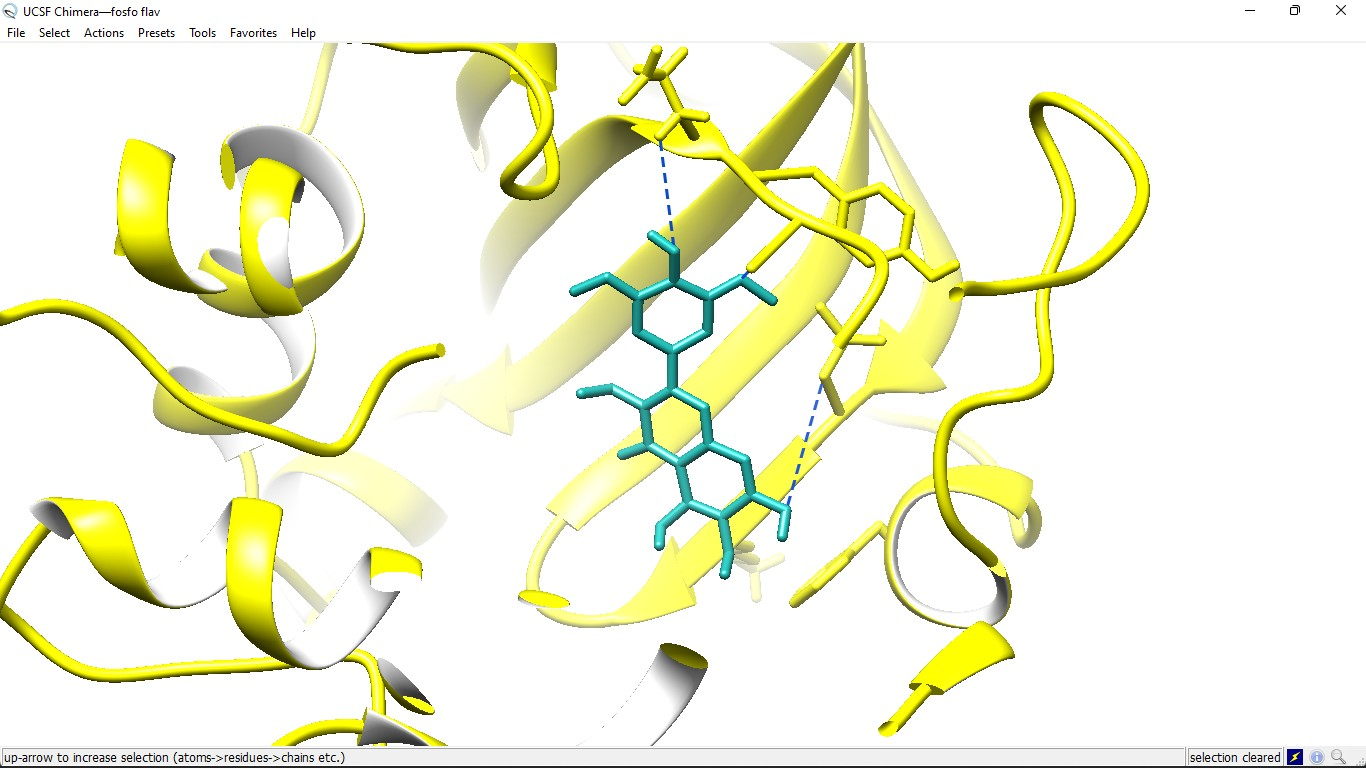
\includegraphics[width=0.65\textwidth]{chimera}
	\end{SCfigure}

        \par{\textbf{Step by step}}
        \par{A basic following steps of how to dock with this program is shown below:}
            \begin{enumerate}[1.]
            \item Once you have your protein and ligand, open the USCF Chimera program.
            \item Then open your files in the program. It will be necessary to add the protonation states and charges assignation.
            \item Save the files previously charged and protonated with extension .mol2.
            \item Run the molecular docking through AutoDock Vina.
            \item Save the obtained poses with the extension .pdb.
            \end{enumerate} 
\subsubsection{ArgusLab}
        \par ArgusLab is a free license program with a user-friendly graphical interface. It is a viewer and editor of biological structures or organic molecules and allows to do molecular docking. The advantage of ArgusLab, over other programs of its type, is that it incorporates parameters of force fields for several metals such as Ni, Cu, Ti, Co, Mn, and more. In such a manner, the diversity of ligands and receptors can be studied using molecular docking studies.
        
\begin{SCfigure}[0.65][ht]
	    \centering
		\caption{Complex protein-bond visualisation in ArgusLab  \cite{Thompson_2004}}
		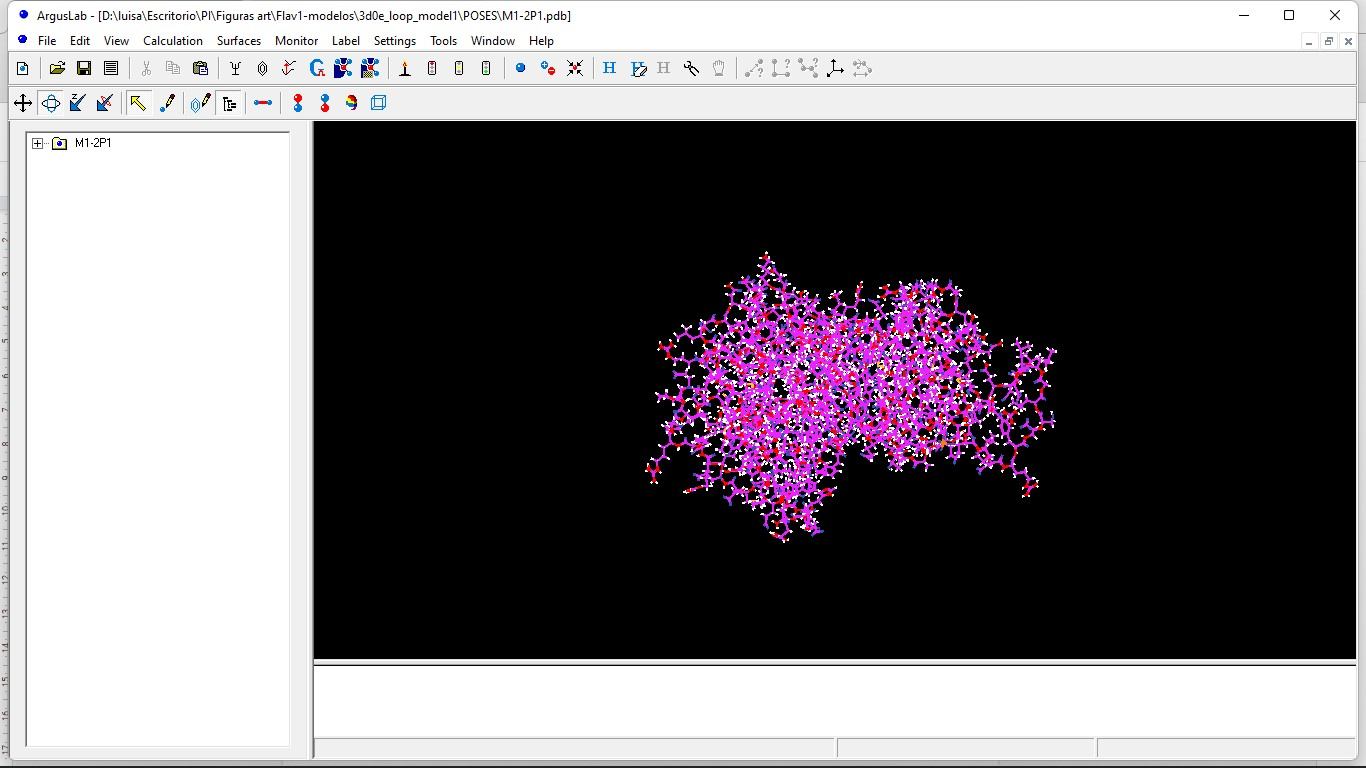
\includegraphics[width=0.65\textwidth]{argus}
	\end{SCfigure}     
	\par{\textbf{Step by step}}
        \par{A basic following steps to consider of how to dock with this program is shown below:}
            \begin{enumerate}[1.]
            \item Once you have your protein and ligand, open the ArgusLab program.
            \item Open your files in the program.
            \item Delete the water molecules by shift + click on the last water molecule/right click/delete.
            \item Select the binding site amino acids and make a group with them. Then do the same with your ligand.
            \item Run the molecular docking with the Calculation/Dock a Ligand option.
            \item Save the results in the .pdb extension.
            \end{enumerate}

        \subsubsection{PyRx}
        \par PyRx is a program that allows molecular docking between proteins and small bonds through AutoDock Vina. Moreover, you can have a basic visualisation of the molecules.
       
\begin{SCfigure}[0.65][ht]
	    \centering
		\caption{Complex protein-bond visualisation in PyRx  \cite{Dallakyan_2014}}
		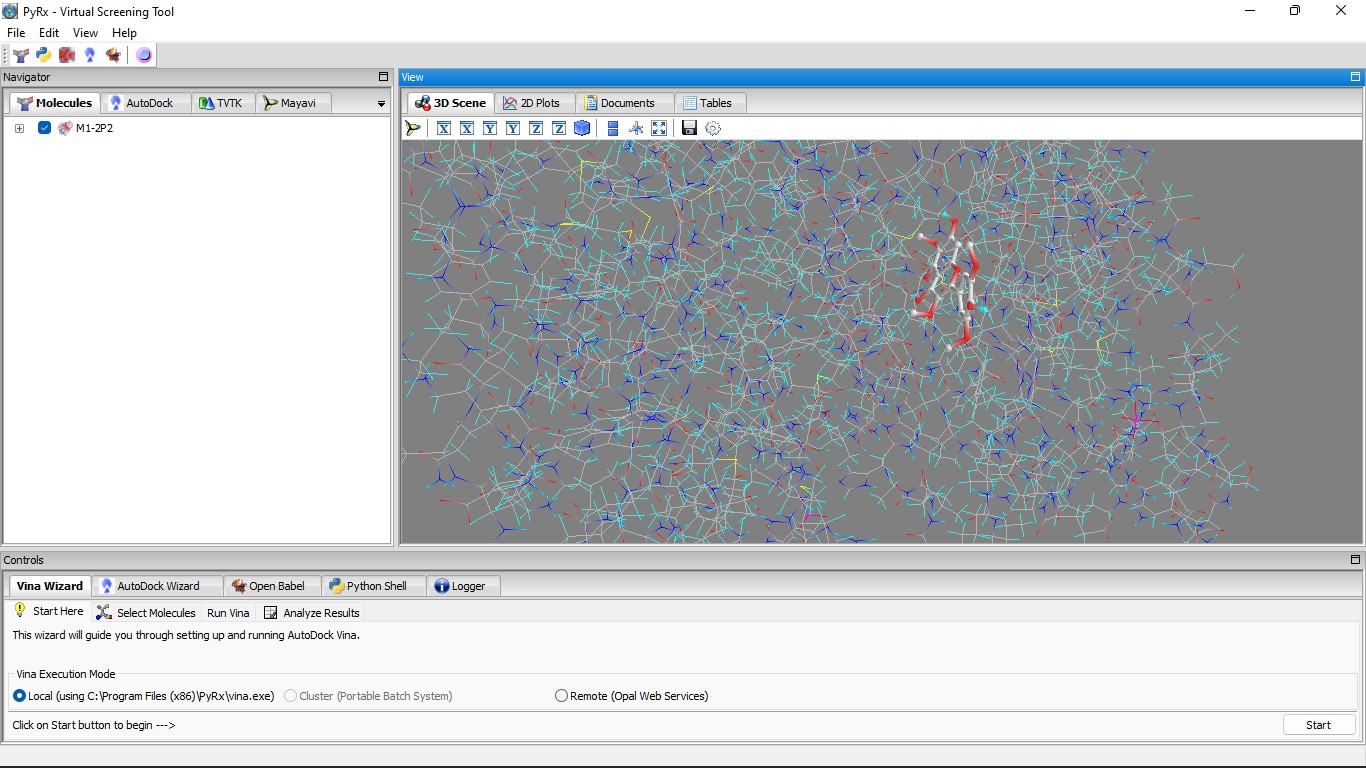
\includegraphics[width=0.65\textwidth]{pyrx.jpg}
	\end{SCfigure}
	
    \par{\textbf{Step by step:}}
    \par{The basic following steps of how to dock with this program are shown below:}
            \begin{enumerate}[1.]
            \item Once you have your protein and ligand, open PyRx.
            \item Open your files in the program in the AutoDock/Vina Wizard section.
            \item Set the molecular docking box conditions.
            \item Run the molecular docking.
            \iteclickve The results in .pdb extension.
            \end{enumerate}

        \subsubsection{Swiss-Model}
        \par Swiss-Model is a fully automated protein structure homology-modelling server, accessible via the Expasy web server or the program DeepView (Swiss Pdb-Viewer). The purpose of this server is to make protein modelling accessible to all life science researchers worldwide.
        
        \par \textbf{Step by step:}
            \begin{enumerate}
                \item Selection of the template protein.
                \par  Should be selected as the best template. Criteria for choosing the structure used as a reference remain the same as in the MODELLER steps. Pay attention to the identity value ($>$ 25\%) between the sequences, best coverage, low E-value, and best crystallographic resolution (the smaller, the better).
               \item Alignment and model building.
               \par SWISS-MODEL already works on the alignment internally. You only need to select the model from the given pick list, and the server fetches the PDB file. The model is then built based on the template and alignment after clicking on "Build Models". We can see that SWISS-MODEL automatically deletes the signal peptide region and does not allow the insertion of the signal peptide.
                \item Model Evaluation
                \par SWISS-MODEL has its evaluation tools. To evaluate the model we should pay attention to the QMEAN (Qualitative Model Energy Analysis) and GMQE (Global Model Quality Estimation) values. QMEAN is an estimator known as the z-score. When the z-value is close to zero it means that the model is considered reliable. Therefore there is good agreement between the model and experimental structures of similar size. The geometric properties provide an estimate of the overall absolute quality. The GMQE, on the other hand, is in a range of 0 to 1. The higher it is, the more accurate the model is for target-model alignment and coverage. SWISS-MODEL also provides an interactive Ramachandran plot on the web page. The Ramachandran plot statistic is 96.72\% of the residuals in favourable regions. After downloading the model, a visual comparison between the template and model structures can be made by structural alignment using the PyMOL tool.
            \end{enumerate}

\subsubsection{CHARMM-GUI}
        \par Among various web-based modelling tools, CHARMM-GUI, [http://www.charmm-gui.org], sets out to simplify and generalize the protocols for building complex simulation systems and preparing simulation input files for widely used simulation packages, such as CHARMM, NAMD, GROMACS, AMBER, GENESIS, LAMMPS, Desmond, OpenMM and CHARMM/OpenMM to facilitate the usage of usual and advanced simulation techniques \cite{Jo_2017}.
     
        
        \par Since its development in 2006, CHARMM-GUI has expanded to a range of capabilities and now contains several different modules designed to configure a wide range of biological systems (Fig. 1) \cite{Jo_2017}.
        
        \par The workflow implemented on the HDOCK server is shown in Figure 8.
        \begin{SCfigure}[0.65][ht]
	    \centering
		\caption{Schematic view of modules in CHARMM-GUI input Generator. [Colour figure can be viewed at willeyonlinelibrary.com]\cite{Jo_2017} )}
		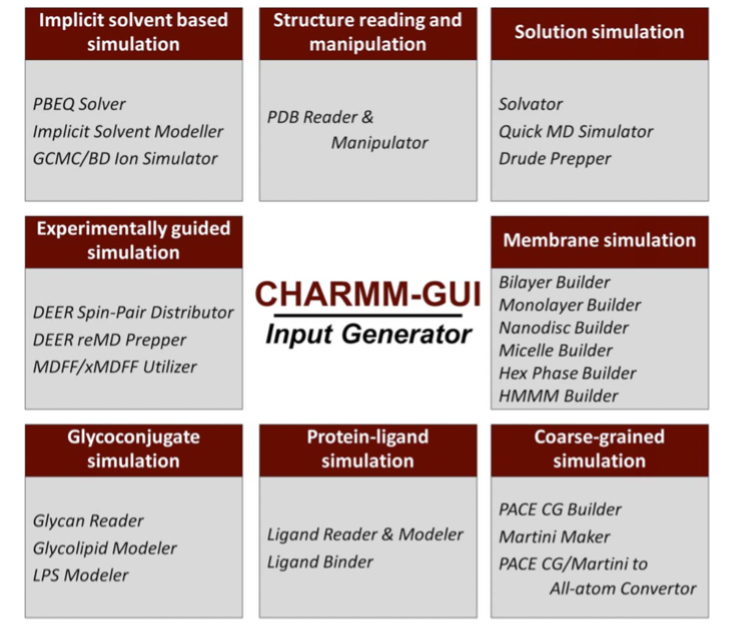
\includegraphics[width=0.65\textwidth]{images/Imagen 1.png}
	\end{SCfigure}\textbf{}
        
        \par The philosophy in the development of CHARMM-GUI is not just about providing the essential elements of molecular modelling but also helping users to perform a task. For example, building a membrane system or dissolving a protein by adding an optimized interface this will makes CHARMM-GUI accessible to users with less experience in modelling tools and yet useful for experts, especially for batch generation of systems. \cite{Jo_2017}.
        
       \par A crucial limitation is that CHARMM-GUI contains many default parameters (e.g., the number of steps for minimizing or the details of how to solvate a protein), which are hidden from users and can make CHARMM-GUI less attractive to more advanced users for their specific customization needs \cite{Jo_2017}. 

\subsubsection{HDOCK}
		\par {Proteins and nucleic acids are the two most important types of biological macromolecules in the cell. Their interactions are crucial for many biological processes like signal transduction, cell regulation, protein synthesis, DNA replication and repair, RNA transcription and others. Therefore, the determination of their complex structures is valuable to understand the biological process at the atomic level and thus develop therapeutic interventions or drugs targeting these interactions. Given the high cost and technical difficulties in experimental methods, molecular docking, which computationally predicts the complexity of individual structures, has been playing a significant role in the determination of complex arrangement \cite{Yan_2017}. To make automatic use as concerns the binding information from the PDB in the dock, HDOCK is a helpful web server.}
		
   \par {The HDOCK server (http://hdock.phys.hust.edu.cn/) is a highly integrated suite of homology search, templated-based modelling, structure prediction, macromolecular docking, biological information, and job management for robust and fast protein-protein docking. The HDOCK server (http://hdock.phys.hust.edu.cn/) is a highly integrated follow of homology search, templated-based modelling, structure prediction, macromolecular docking, biological information, job management for robust and fast protein-protein docking. It distinguishes by using Amino Acids sequences as input and a hybrid docking strategy where experimental information (about the protein-protein binding site) and small-angle X-ray scattering can be incorporated during the docking and the post-docking processes. The server also supports protein-RNA/DNA docking with an intrinsic scoring function. It provides the template and the docking-based binding models of two molecules and allows for the download of interactive visualization. The HDOCK server is used and has processed >30,000 docking jobs since its official release in 2017.  The server can commonly complete a docking job within 30min \cite{Yan_2020}}

		\par {The workflow implemented on the HDOCK server is shown in Figure 9.}
        \begin{SCfigure}[0.65][ht]
	    \centering
		\caption{The workflow of the HDOCK web server is divided into four stages: (1) data input, (2) sequence similarity search, (3) structure modelling and (4) FFT-based global docking in which priority is given to user-input structures. ] \cite{Yan_2017})}
		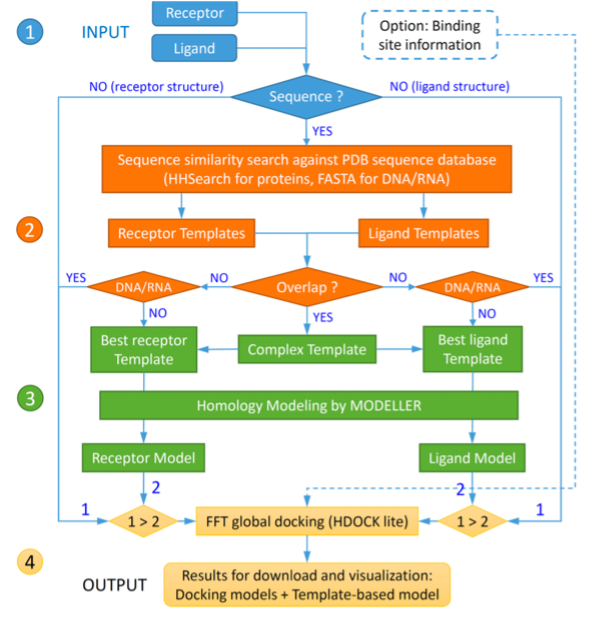
\includegraphics[width=0.65\textwidth]{Imagen 2.png}
	\end{SCfigure}\textbf{}

\par According to \cite{Jo_2017} to best facilitate the use of the HDOCK server by normal users, especially for non-expert users, the server is designed to accept both sequence and structure inputs for proteins, two for structures and two for sequences, as follows:
1)	Upload your pdb file in PDB format.
2)	Provide your pdb file in PDB ID: ChainID (e.g., 1CG1: E). 
3)	Copy and post-docking protein sequence below in FASTA format.
4)	Upload your protein sequence file in FASTA format.

\subsubsection{GLYCAM-Web}
Many research areas of docking-based focused on structural aspects of biomolecules “moved into cyberspace” in the past 20-30 years have become even more prominent. Amplified by the increased space accessibility (from mobile devices to the cloud) and even more sophisticated and powerful resources available for high-performance computing. Structural glycobiology has greatly modelled from such progress and has taken advantage of the computational tools and resources developed specifically for the structural analysis of carbohydrates \cite{Yuriev_2015}.
GLserverWeb target the prediction of three-dimensional carbohydrates and macromolecular structures, including carbohydrates. 
The server is created and operated by the research group of Prof. Robert J. Woods in the Complex Carbohydrate Research Center (CCRC) at the University of Georgia, Athens. This server can perform conformational modelling of oligosaccharides by counting the 3D modelling of glycoproteins.  
It is crucial to mention that:
1. the Carbohydrate Builder, including a crucial builder for glycosaminoglycans (GAGs)
2. the Glycoprotein Builder, 
3. and the Oligosaccharide Libraries are relevant attachments to model the oligosaccharide conformation. The server is user-friendly and allows a range of upload and download options.
Already given a range of file formats, program-specific used in molecular modelling, user-friendliness related to the portability of file formats is a significant “real-estate” feature highly valued by cyberspace dwellers \cite{Yuriev_2015}.

    \subsection{Molecular interactions simulation tools}
                \subsubsection{GROMACS}
        \par{GROMACS is an open-source, cross-platform program for performing molecular dynamics simulations and energy minimization of systems with hundreds of millions of particles. It allows knowing and predicting the behaviour of macroscopic properties through the description of complex chemical systems in terms of a realistic atomic model.}
        \par{Checking a small example \cite{Villa_2017}, we will see the visualization of a small protein (Factor Xa, PDB code:v1FJS), which is a protein that generates blood clots. For visualization:}
        \\
        
        \par{import nglview as ng}
        \par{$view = ng.show_structure_file("input/1fjs.pdb")$}
        \par{view}
        \\
        
        \par{This way we can see an image like the one in Figure 3.}
        \begin{SCfigure}[0.65][ht]
	    \centering
		\caption{Factor Xa visualization (From: \cite{Villa_2017})}
		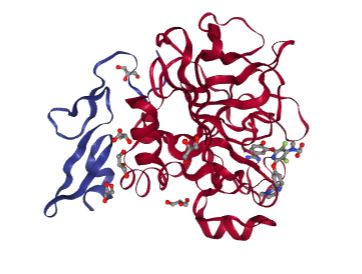
\includegraphics[width=0.65\textwidth]{Proteina.JPG}
	\end{SCfigure}
	
\par{However, this visualization contains atoms that do not correspond to the protein structure. To remove these atoms (called "HETATM" in the PDB file), it's a matter of using grep:}

\vspace{0.5 cm}

\par{$!grep -v HETATM input/1fjs.pdb > 1fjs_protein_tmp.pdb$}
\par{$!grep -v CONECT 1fjs_protein_tmp.pdb > 1fjs_protein.pdb$}
\par{To visualise it:}
\par{Import nglview as ng}
\par{$view = ng.show_structure_file("1fjs_protein.pdb")$}
\par{view}
\\

\par{Thus we obtain a purer structure such as in Figure XXX:}

\begin{SCfigure}[0.65][ht]
	    \centering
		\caption{Factor Xa pure visualisation (From\cite{Villa_2017})}
		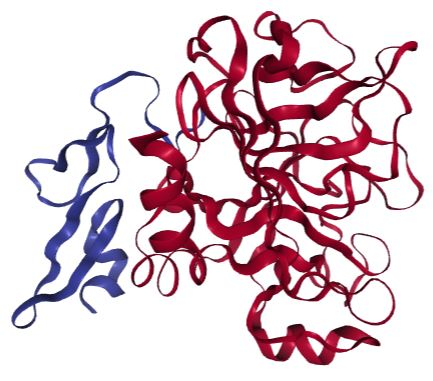
\includegraphics[width=0.5\textwidth]{ProteinaPura.JPG}
	\end{SCfigure}


\subsubsection{AutoDocks}
\par{Autodock is one of the most widely used molecular model simulation software designed to predict the binding between small molecules and receptors with known three-dimensional structures. The calculations carried out are developed in 4 main steps:}
\vspace{0.4 cm}

\par{Coordinate File Preparation. 
During this stage, the ligand and receptor are able to include the information needed to use AutoDock. For this, PDBQT type files are used, including polar hydrogen atoms, partial charges,  types of atoms, and information about the flexibility of molecules. To generate files it is possible to use AutoDockTools.}
    \par{Running AutoGrid.
 Running AutoDock requires a precomputed grid map for each type of atom in the docking ligand. These maps consist of a three-dimensional network of regularly spaced points that surround a region of interest in the macromolecule that has been studied. To start AutoGrid, the following code is used:}
    
\vspace{0.4 cm}
    autogrid4 -p macro.gpf [-l macro.glg]
\vspace{0.4 cm}

    \par{Molecular docking with AutoDock. AutoDock evaluates the protein-ligand interactions at each point using a cluster simulation. For this, AutoDock requires a map calculated by AutoGrid, a ligand in PDBQT format, and a parameter file for clustering. The calculations start with the following code:}
\vspace{0.4 cm}

autodock4 [-i][-u][-t] -p lig.dpf [-l lig.dlg]

\vspace{0.4 cm}

\par{Results evaluation.
At the end of the simulation, the coordinates are obtained for each point where the binding was formed. Then, the information on the formation of clusters and interaction energies. The data processing is done in the “Analyze” section in the AutoDockTools menu.}

\newpage

\subsubsection{ClusPro} %02/10/2022

\par{The ClusPro server is used for the structural analysis of a protein-protein docking and the results obtained can allow the identification of the best docking conformations. ClusPro features a basic user interface but also allows applying several advanced options in the search, such as removing unstructured protein regions, applying attraction or repulsion, accounting for pairwise distance constraints, constructing homomultimers, and locating heparin binding sites (Kozakov et al., 2017). The execution of the analyses on the server is performed following three computational steps (Kozakov et al., 2017):} 

\begin{enumerate}
    \item Rigid body fitting by sampling billions of conformations;
    \item Clustering based on the root mean square deviation (RMSD) of the 1,000 lowest energy structures generated, to find the largest clusters that will represent the most likely models of the complex;
    \item Refinement of selected structures using energy minimisation.
\end{enumerate}

\subsubsection{PIPER}

\par{PIPER is a fitting program based on the Fast Fourier Transform (FFT) correlation approach and is used in the rigid body fitting step. A receptor protein is placed at the origin of the coordinate system on a fixed grid, while a ligand-protein is placed on a moving grid. In this process, the interaction energy is written in the form of a correlation function and the FFT-based algorithm allows protein fitting without prior information about the structure of the complex (Kozakov et al., 2017).}

\subsubsection{PatchDock}

\par{PatchDock uses a technique similar to a jigsaw puzzle. Given two molecules, their surfaces are divided into pieces according to surface shape. These pieces correspond to visually distinguishable patterns. Once the chunks are identified, they can be overlaid using matching shape algorithms. The algorithm has three main stages:}

\begin{enumerate}
    \item Molecular Shape Representation - in this step, the molecular surface of the molecule is calculated. Next, a segmentation algorithm is applied to detect geometric speckles (concave, convex, and flat surface pieces). The pieces are filtered so that only pieces with hot spot residues are retained.
    \item Surface Chunk Matching - a hybrid of the Geometric Hashing and Pose-Clustering matching techniques is ligand-protein chunks detected in the previous step. Concave chunks are matched with convex chunks and planes with any type of chunks.
    \item Filtering and Scoring - the candidate complexes from the previous step are examined. All complexes with unacceptable penetrations from the receptor atoms to the ligand atoms are discarded. Finally, the remaining candidates are ranked according to a geometric shape complementarity score.
\end{enumerate}

\par{The results of PatchDock are presented in a list with the candidate receptor-ligand complexes. The list is presented to the user in a table format, each table row representing a candidate complex}

\par{The parameters used are:}

\begin{itemize}
    \item\textbf{ Solution No:} Number of the candidate complex

    \item \textbf{Score:} Complementarity score of geometric form. The candidate complexes are ordered according to this score.

    \item \textbf{Area:} Approximate interface area of the complex.

    \item\textbf{ACE:} Atomic contact energy

    \item \textbf{Transformation 3D:} 3 rotation angles and 3 translational parameters. The transformation is applied to the ligand molecule.

    \item \textbf{PDB file of the complex:} The predicted complex structure in PDB format.
\end{itemize}

\subsubsection{FireDock}

\par{As another software for analysis and scoring of protein-protein docking solutions, FireDock uses two options for initial input in its server: a transformation file, which requires an input of the receptor and ligand molecules and the transformation files, following the format of rotations and translations in the X, Y and Z axes; or with a model file, which uses a file containing models of the complexes for analysis and the receptor and ligand chains. The output for obtaining the results, therefore, follows the model table with all the input solutions, ranked by the global energy value, and which has several scoring parameters, namely:}

\begin{itemize}
    \item Rank - related to the overall energy; 
    \item Solution number - related to the order of transformations or models; 
    \item Global energy - the binding energy of the solution; 
    \item Van der Waals attractive and repulsive forces (VdW) and their contribution to the overall binding energy;
    \item Atomic contact energy (ACE) in relation to the overall binding energy and 
    \item The contribution of hydrogen bridges (HB) to the overall binding energy.
\end{itemize}

    \subsubsection{PyDock}

    \par{PyDockWEB is a web server for the rigid-body docking prediction of protein-protein complex structures using a new version of the pyDock scoring algorithm. We use here a new custom parallel FTDock implementation, with adjusted grid size for optimal FFT calculations, and a new version of pyDock, which dramatically speeds up calculations while keeping the same predictive accuracy. Given the 3D coordinates of two interacting proteins, pyDockWEB returns the best docking orientations as scored mainly by electrostatics and desolvation energy.}

    \par{PyDockWEB server is a web application for the use of the protein-protein docking and scoring program pyDock. Users can easily send pyDock jobs to be executed in a five-step process via a user-friendly frontend. In the first step, users have to introduce a project name and a notification email address. In the second step, the scoring algorithm is selected. In the third step, users can either upload their protein coordinate files or indicate the PDB code, in which case, PDB files will be automatically downloaded from RCSB Protein Data Bank. In both cases, PDB files are automatically parsed to select available receptor and ligand chains. An option to automatically set up a docking job with example PDB files is also available. In the fourth step, users may specify optional distance restraints, which will be computed using the pyDockRST module. Finally, in the fifth step, users will double-check whether the data provided are correct and submit a docking job to the server queues. After job submission, the user is redirected to a web page where the project status is automatically updated and the result files can be downloaded after the computation is finished. On this web page, the top 10 models scored by PyDock are displayed using Jmol.}

\begin{itemize}
    \item  \textbf{Parameters:} Electrostatics, Desolvation, VdW (Van der Waals)
\end{itemize}
   
    \par{The scheme is based on Coulombic electrostatics with a distance-dependent dielectric constant, and implicit desolvation energy with atomic solvation parameters previously adjusted for rigid-body protein-protein docking. This scoring function is not highly dependent on the specific geometry of the docking poses and therefore can be used in rigid-body docking sets generated by a variety of methods. We have tested the procedure in a large benchmark set of 80 unbound docking cases. The method is able to detect a near-native solution from 12,000 docking poses and place it within the 100 lowest-energy docking solutions in 56\% of the cases, in a completely unrestricted manner and without any other additional information. More specifically, a near-native solution will lie within the top 20 solutions in 37\% of the cases. The simplicity of the approach allows for a better understanding of the physical principles behind the protein-protein association, and provides a fast tool for the evaluation of large sets of rigid-body docking poses in search of the near-native orientation.}
    

    
    
    

\subsection{Parameters used in modelling} %%02/10/2022

    \par{In structural modelling, there are several parameters used by different software to express mathematically how close their result is to the protein structure. They are also necessary for further calculations.}

\subsubsection{C-Score}

    \par{C-score is a confidence score for estimating the quality of predicted models by I-TASSER. It is calculated based on the significance of threading template alignments and the convergence parameters of the structure assembly simulations. C-score is typically in the range of [-5,2], where a C-score of higher value signifies a model with high confidence and vice-versa.}

\subsubsection{TM-Score}

    \par{TM-score is a recently proposed scale for measuring the structural similarity between two structures. The purpose of recommending a TM-score is to solve the problem of RMSD which is sensitive to local error. Because RMSD is an average distance of all residue pairs in two structures, a local error (e.g. a misorientation of the tail) will arise a big RMSD value although the global topology is correct. In TM-score, however, the small distance is weighted stronger than the distance which makes the score insensitive to the local modelling error. A TM-score >0.5 indicates a model of correct topology, and a TM-score<0.17 means a random similarity. This cutoff does not depend on the protein length.}

\subsubsection{Cluster density}

    \par{I-TASSER generates a full-length model of proteins by excising continuous fragments from threading alignments and then reassembling them using replica-exchanged Monte Carlo simulations. Low-temperature replicas (decoys) generated during the simulation are clustered by SPICKER and the top five cluster centroids are selected for generating full atomic models. The cluster density is defined as the number of structure decoys at a unit of space in the SPICKER cluster. A higher cluster density means the structure occurs more often in the simulation trajectory and therefore signifies a better-quality model. The values in the second last column of the above-mentioned table represent the number of structural decoys that are used in generating each model. The last column represents the density of the cluster.}

\subsubsection{ERRAT}

    \par{Analyses the statistics of non-bonded interactions between different atom types and plots. The value of the error function versus the position of a 9-residue sliding window is calculated by comparison with statistics from highly refined structures.}

    \par{A novel method for differentiating between correctly and incorrectly determined regions of protein structures based on characteristic atomic interaction is described. Different types of atoms are distributed non-randomly concerning each other in proteins. Errors in model building lead to more randomized distributions of the different atom types, which can be distinguished from correct distributions by statistical methods. Atoms are classified into three categories: carbon (C), nitrogen (N), and oxygen (O). That leads to six combinations of pairwise non-covalent bonded interactions (CC, CN, CO, NN, NO, and OO). A quadratic error function is used to characterize the set of pairwise interactions from nine-residue sliding windows in a database of 96 reliable protein structures. Regions of candidate protein structures that are mist-raced or misregistered can then be identified by analysis of the pattern of non-bonded interactions from each window.}

\subsubsection{Verify 3D}

    \par{Determines the compatibility of an atomic model (3D) with its own amino acid sequence (1D) by assigning a structural class based on its location and environment (alpha, beta, loop, polar, non-polar etc) and comparing the results to good structures.}
    
    \par{The inverse protein folding problem. The problem of finding which amino acid sequences fold into a known three-dimensional (3D) structure, can be effectively attacked by finding Amino Acids sequences compatible with the environments of the residues in the 3D structure. The situation is described by: 
(i) the area of the residue buried in the protein and inaccessible to solvent; 
(ii) the fraction of the side-chain area that is covered by polar atoms (O and N); and 
(iii) the local secondary structure. 
Examples of this 3D profile method are presented for four families of proteins: the globins, cyclic AMP (adenosine 3',5'-monophosphate) receptor-like proteins, the periplasmic binding proteins, and actins. This method can detect the structural similarity of the actions and 70- kilodalton heat shock proteins, even though these protein families share no detectable sequence similarity.}

    \par{As methods for determining protein three-dimensional (3D) structures develop, a continuing problem is how to verify that the final protein model is correct. The revision of several protein models to correct errors has prompted the development of new criteria for judging the validity of X-ray and NMR structures, as well as the formation of energetic and empirical methods to evaluate the correctness of protein models. The challenge is to distinguish between a mist-raced or wrongly folded model and one that is correct, but not adequately refined. We show that an effective test of the accuracy of a 3D protein model is a comparison of the model to its amino-acid sequence, using a 3D profile, computed from the atomic coordinates of the structure 3D profiles of correct protein structures match their sequences with high scores. In contrast, 3D profiles for protein models are known to be wrong and score poorly. An incorrectly modelled segment in an otherwise correct structure can be identified by examining the profile score in a moving-window scan. The accuracy of a protein model can be assessed by its 3D profile. Regardless of whether the model has been derived by X-ray, NMR, or computational procedures.}

\subsubsection{PROVE (z-score)}

    \par{Calculates the volumes of atoms in macromolecules using an algorithm that treats the atoms like hard spheres and calculates a statistical Z-score deviation for the model from highly resolved (2.0 Å or better) and refined (R-factor of 0.2 or better) PDB-deposited structures.}

    \par{Standard ranges of atomic and residue volumes are computed in 64 highly resolved and well-refined protein crystal structures using the classical Voronoi procedure. Deviations of the atomic volumes from the standard values, evaluated as the volume Z-scores, are used to assess the quality of protein crystal structures. To score an arrangement globally, we compute the volume Z-score root mean square deviation (Z-score RMS), which measures the average magnitude of the volume irregularities in the structure. We find that the Z-score RMS decreases as the resolution and R-factor improve, consistent with the fact that these improvements generally reflect more accurate models. From the Z-score RMS distribution in structures with a given resolution or R-factor, we determine the normal limits in Z-score RMS values for structures solved at that resolution or R-factor. Conformations whose Z-score RMS exceeds these limits are considered outliers. It also exhibits unusual stereochemistry, as revealed by other analyses. Absolute Z-scores of individual atoms are used to identify problems in specific regions within a protein model. These Z-scores correlate reasonably well with the atomic B-factors, and atoms having absolute Z-scores > 3, occur at or near sectors in the model where programs such as PROCHECK identify unusual stereochemistry. Atomic volumes, themselves not directly restrained in crystallographic refinement, can thus provide an independent, adequately sensitive, measure of the quality of a protein structure. The volume-based structure validation procedures are implemented in the program PROVE (Protein Volume Evaluation), which is accessible through the World Wide Web.}

\subsubsection{PROCHECK -  Ramachandran plot}

    \par{Checks the stereochemical quality of a protein structure by analyzing residue-by-residue geometry and overall structure geometry.}

    \par{These Operating Instructions describe how to run the PROCHECK suite of programs (Laskowski et al., 1993) for assessing the "stereochemical quality" of a given protein structure. PROCHECK aims to assess how usual or atypical the geometry of the residues in a given protein structure is,  compared with stereochemical parameters derived from well-refined, high-resolution structures. Rare regions highlighted by PROCHECK are not necessarily errors as such but may be unusual features for which there is a reasonable explanation (e.g. distortions due to ligand-binding in the protein's active site). Nevertheless, they are regions that should be checked carefully.}

    \par{The stereochemical parameters used are those described in detail in Morris et al. (1992). These parameters, which are for the most part not included in standard refinement procedures (and so are less likely to be biased by them), are listed in Table 1 of Appendix A. The checks also make use of "ideal" bond lengths and bond angles, as derived from a recent and comprehensive analysis (Engh \& Huber, 1991) of small molecule structures in the Cambridge Structural Database, CSD (Allen et al., 1979) - now numbering over 100,000 structures. These "ideal" values are listed in Table 2 of Appendix A.}

    \par{Methods have been developed to assess the stereochemical quality of any protein structure both globally and locally using various criteria. Several parameters can be derived from the coordinates of a given structure. Global parameters include the distribution of phi, psi and chi one torsion angles, and hydrogen bond energies. There are clear correlations between these parameters and resolution; as the resolution improves, the distribution of the parameters becomes more clustered. These features show a broad distribution of ideal values derived from high-resolution structures. Some structures have tightly clustered distributions even at relatively low resolutions, while others show abnormal scatter though the data go to high resolution. Additional indicators of local irregularity include proline phi angles, peptide bond planarities, disulfide bond lengths, and their chi-three torsion angles. These stereochemical parameters have been used to generate measures of stereochemical quality. It provides a simple guide as to the reliability of a structure. In addition, the most critical measures are resolution and R-factor. The parameters used in this evaluation are not novel and are easily calculated from structure coordinates. A program suite is currently being developed to quickly check a given structure, highlighting unusual stereochemistry and possible errors (Stereochemical quality of protein structure coordinates).}


\newpage 
\section{Control statements}
\subsection{Introduction}
\par{Control statements allow you to control the flow of the program, making decisions based on comparisons and generating loops while or until certain conditions are met. A conditional or selection statement (or structure) is one that establishes which statements should be executed or not, depending on the value of a condition. There are three main types of conditionals: single condition (if), biconditional (if-else), or multiple condition (switch-case-default)} \cite{iscyp_2017}.
    \subsection{Characteristic Commands}
    \vspace{1 cm}
    \underline{Simple conditional statement}
   \\
    \\
    \textbf{IF}
    \par{A simple conditional is a control structure that executes a set of lines of code if a Boolean expression is true. The general format of an if statement is as follows \cite{tiwari_2022}}.
    \\
    \\
    if (condition) \{ \{
    
    instruction 1
     \\
     ...
     \\
     instruction 2
     \\
     Lines of code are executed if the expression is true.
     \\
     Otherwise, they are not executed
     \\
\
\}
\}
\\
\par{If the expression is evaluated to nonzero (true) then if block statement(s) are executed. If the expression is evaluated to zero (false) then Control passes to the next statement following it \cite{tiwari_2022}.}
\\
%%la imagen no se imprime correctamente
\begin{SCfigure}[0.8][ht]
	    \centering
		\caption{If statement, (Obtained from: {DotNetTricks})}
		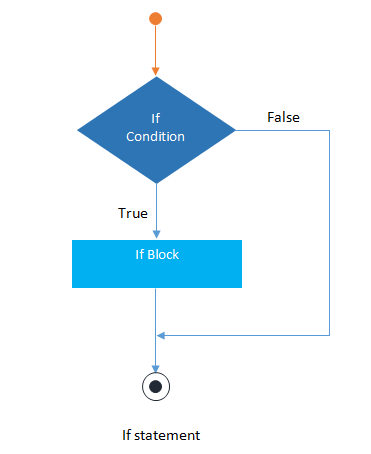
\includegraphics[width=0.2 \textwidth]{ifstatement.png}
		\label{Imagen_if}
	\end{SCfigure}
	
\underline{Double conditional instruction}
\\
\textbf{IF-ELSE}

\par{The if/else statement extends the if statement by specifying an action if the if (true/false expression) is false.}
\par{An else clause can be added to a simple conditional to specify which lines of code to execute if the boolean expression is false. In this case, we are talking about the if-else structure, which in Processing is expressed according to this code \cite{iscyp_2017}.}
\\
if (condition)\\
\{ \\
   do this if the condition is true\\
   if true statements\\
\} \\
else \\
\{ \\
   do this if the condition is false \\
   if false statements \\
\}
\par{With the if statement, a program will execute the true code block or do nothing. With the if/else statement, the program will execute either the true code block or the false code block so something is always executed with an if/else statement \cite{iscyp_2017}.}
\begin{itemize}
    \item If the expression is evaluated to nonzero (true) then, the if block statement(s) are executed.
    \item{If the expression is evaluated to zero (false) then, the else block statement(s) are executed.}
\end{itemize}
\begin{SCfigure}[0.8][ht]
	    \centering
		\caption{If-else-ladder, (Obtained from: {DotNetTricks})}
		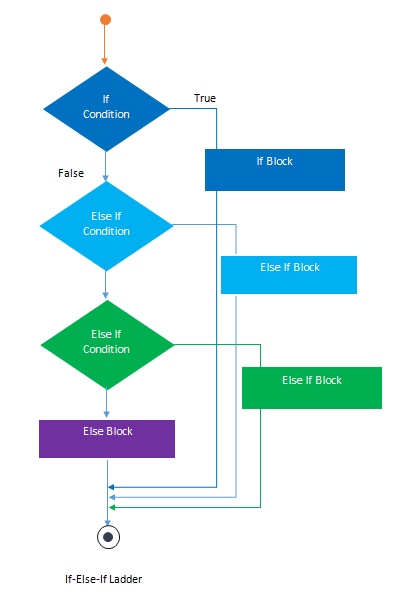
\includegraphics[width=0.2 \textwidth]{if-else-if ladder.png}
		\label{Imagen_If-else}
	\end{SCfigure}
	
\vspace{0.5 cm}
\underline{Multiple conditional statement}\\
\textbf{SWITCH}
\par{Allows a variable to be compared with different possible values, executing a series of specific instructions for each case. The switch statement acts as a substitute for a long if-else-if ladder that is used to test a list of cases. A switch statement contains one or more case labels that are tested against the switch expression. When the expression match a case then the associated statements with it would be executed.
\\
If-else ladder, but the need for an additional way of dealing with conditional statements may seem unnecessary but based on the certain usage, switch case was defined to check for the single condition, and based on the multiple cases, code can be executed.}
\vspace{0.5 cm}
Switch (expression) \{ \\
   case value1: \\
     // Statements are executed when the result of the expression 
     
     matches value 1
     
     [break;] 
     
     \vspace{0.5 cm}
     
   case value 2: \\
     // Statements executed when the result of expression \\ matches value 2 \vspace{0.5 cm}
     [break;] 
   ... \\
   case value n:\\
     // Statements executed when the result of expression \\ matches value n \vspace{0.5 cm}
     [break;] \\
   default: \\
     // Statements executed when none of the values match the \\ value of the expression \vspace{0.5 cm}
     [break;] \\
\} \\

\begin{SCfigure}[1][ht]
	    \centering
		\caption{Switch statement, (Obtained from: {DotNetTricks})}
		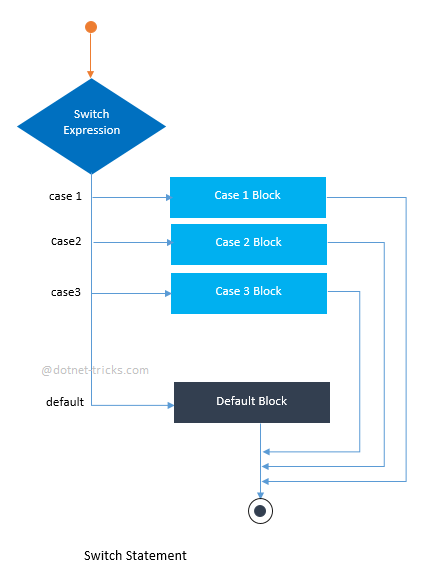
\includegraphics[width=0.5 \textwidth]{switch.png}
		\label{Imagen_Switch}
	\end{SCfigure}
	
\par{A couple of observations about this structure:
\begin{itemize}
\item At least one case is required.
\item If you are going to use a few cases, you might want to consider using nested if-else instead of switch-case.
\item The default clause is optional. You are not obliged to put it, but it is advisable.
\item The statement break; prevents Processing from executing the following lines of the following case.
\end{itemize}
\par{For example, if the first break had not been set in the example above, then the messages "Monday" and "Tuesday" would be displayed. The following example should clarify this aspect for you}}\\ \\
\textbf{WHILE}
\par{They are used when we want to repeat the execution of statements an indefinite number of times, as long as a condition is met. It is easier to understand than the FOR loop since it does not incorporate the initialisation of the variables, their condition to continue executing and their updating on the same line. It only indicates, as we will see below, the condition that must be fulfilled for an iteration to be carried out.}\\
   \begin{itemize}
       \item The condition will always be evaluated before each iteration.
       \item The body of the while loop repeats as long as the condition is true.
       \item The body of a while loop will execute zero or more times.
   \end{itemize}
   \par{An expression that is evaluated before each step of the loop. If this condition evaluates to true, the statement is executed. When the condition evaluates to false, execution continues with the statement after the while loop.} \\
   
   \begin{SCfigure}[1][ht]
	    \centering
		\caption{While statement, (Obtained from: {DotNetTricks})}
		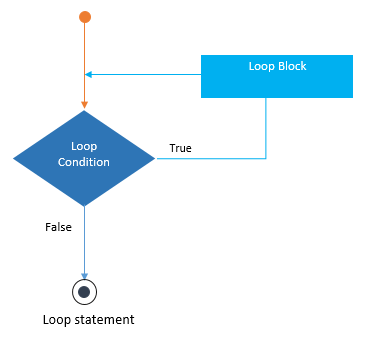
\includegraphics[width=0.2 \textwidth]{cloop.png}
		\label{Imagen_while}
	\end{SCfigure}
	\par{Typically, while loop is useful when you are not aware of an exact number of iterations.}\\
	
    \underline{Repetitive control statement}\\
    \textbf{DO-WHILE}\\
    \par{Is used to execute a block of instructions at least once. The body of the loop is repeated while the condition is checked. This condition will be evaluated after each repetition. A program can be built by using one of the loop statements. For example, we can print numbers from 1 to 100 using all loops.}\\ \\
    do\\
    \{ \\
    instruction 1 \\
    ... \\
    instruction n\\
    \} while (condition); \\
    \par{Typically, for loop, is useful when you are aware of the exact number of iterations. Normally, it is used for iterating over arrays and for sequential processing.}
    
    \begin{itemize}
\item The body of a do-while loop will execute one or more times.
\item The body of the do-while loop is repeated as long as the condition is true.
\item The condition will always be evaluated after each iteration.
\end{itemize} \vspace{0.5 cm}
\textbf{For} \vspace{0.5 cm}
\par{It is used to execute a block of instructions a fixed number of times that is known in advance. The for loop is most convenient with counting loops. Loops that are based on a counting variable are used to have a known number of iterations. The statement can be a single statement or a compound statement (block), so an alternate way to write the format might be:}\\

    for (initialCondition; testExpression;iterativeStatement)\\ 
 \{\\
    statement1;\\
    statement2;\\
    // ...\\
    statementN;\\
 \}\\
\par{How it works:\\
The initial condition runs once, at the start of the loop
The test Expression is checked. (This is just like the expression in a while loop). If it's false, quit. If it's true,
\begin{itemize}
    \item Then run the loop body
    \item Run the iterative Statement
    \item Go back to the test Expression step and repeat
\end{itemize}
}
    
  \newpage  
  


    
  

    
\newpage

\section{Examples of modelling of biological systems in iGEM}
\par{In this section we show you some examples of mathematical modelling of other equipment in iGEM that can serve as a reference for modelling your project. We invite you to visit the wikis of other teams so that, like us, you will be inspired by the incredible work that other teams have developed.}
    \subsection{Modelling a pathway that helps you decide which promoter to use.}
        \par{The \href{https://2021.igem.org/Team:Vilnius-Lithuania/Model}{Vilnus-Lithuanian 2021 team} performed mathematical modelling to choose pro-motors to modify their organism's metabolic pathway in an optimal way.}
        \par{They began by using simple modelling using Michaelis-Menten kinetics. With this, they simulated the change of product and substrate of their enzymatic reaction with respect to time. In addition, are constructed differential equations to model the concentration of the enzyme of interest and its respective mRNA.}
        \par{Finally, they modelled the Naringenin synthesis pathway using a system of chemical equations. This system was converted to differential equations. And, with the assumptions they made, they were able to simplify the model to a few equations.}
        \begin{SCfigure}[0.65][h]
	    \centering
		\caption{Naringenin synthesis pathway}
		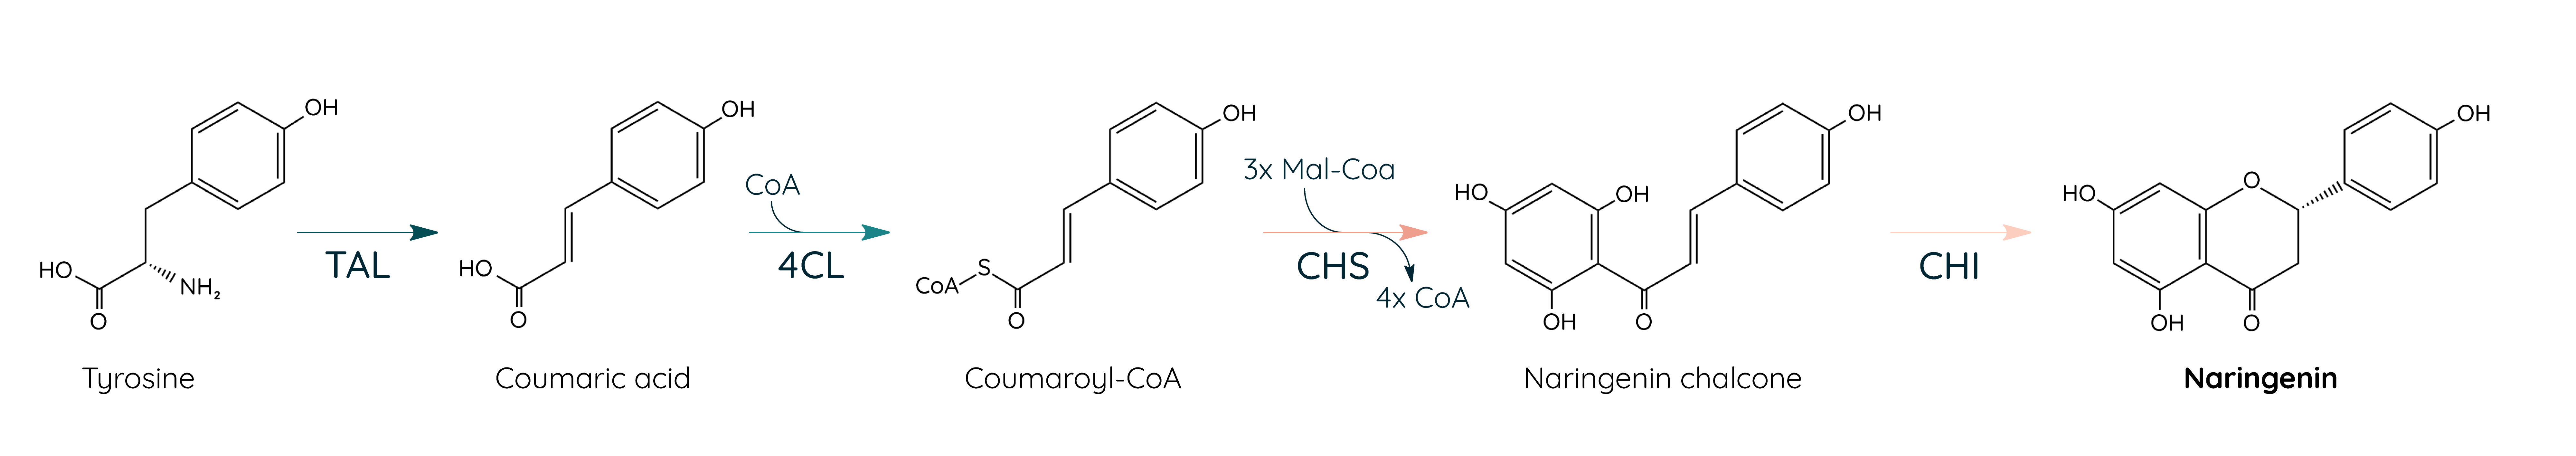
\includegraphics[width=0.65\textwidth]{Vilnus.png}
	\end{SCfigure}
\par{The model helped them to decide which promoter to use, and they were able to determine the bottleneck step in the Naringenin synthesis pathway.}
\subsection{Modelling the time needed to produce a component of interest}
\par {Modelling gene expression with a system of ODEs is a very common task in iGEM projects. A good example of this is the work performed by \href{https://2015.igem.org/Team:Oxford/Modelling#characterising-our-cells}{iGEM Oxford} in 2015. They worked on a project which was focused on making an alternative to antibiotics for the treatment of urinary infections. For this, they engineered \textit{Escherichia coli} to produce enzymes that could break down bacterial biofilms responsible for the generation of urinary infections. Naturally, it was necessary to know if their engineered bacteria could produce the necessary amount of enzymes. This is the part where the maths modelling enters.}

\par {Through a system of ODEs, the team was able to predict the necessary time to produce the desired amount of their protein of interest. Using an arabinose-induced expression system, they used Michaelis-Menten kinetics to generate their system and compare their results with experimental data to fit their data. With these, they were able to calculate the limiting concentrations of their products. A remarkable aspect of this work is the consideration and research of their model parameters, which gives great validity to their model \cite{iGEMOxford_2015}.}

\begin{SCfigure}[0.65][ht]
	    \centering
		\caption{Well-documented parameters validate a team's model and help future teams to build their own systems \cite{iGEMOxford_2015}}
		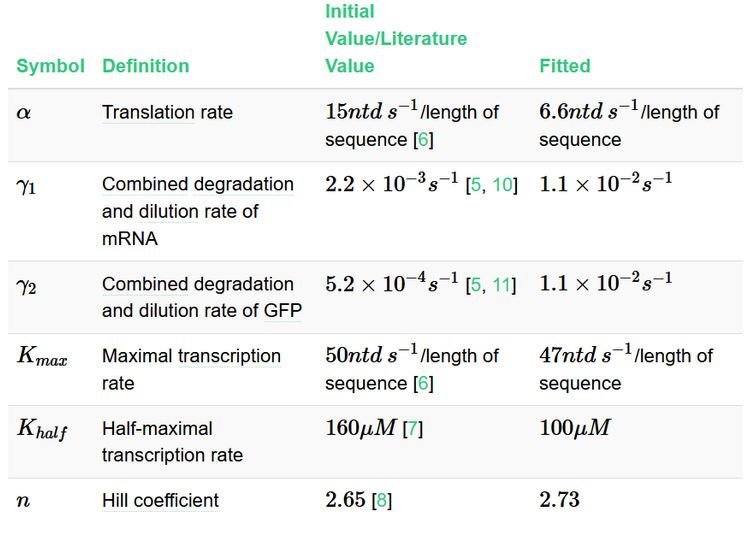
\includegraphics[width=0.65\textwidth]{Tabla parametros.JPG}
	\end{SCfigure}
	\vspace{0.3 cm}
    \subsection{Modelling a Michaelis\texorpdfstring{$-$}{Lg}Menten reaction }
    \par {Another example is the model from the \href{https://2018.igem.org/Team:Queens_Canada/Michaelis-Menten_Kinetics}{Queens Canada 2018 team.} They did several modelling processes but we are going to focus on the Michaelis-Menten Kinetics section that helps in analysing the enzyme kinetic.} 
    \par {In this part, they did a calculator that works with the inputs of substrate concentration, product concentration and enzyme concentration. This information is put on a function that generates the rate of change of concentration. This program was made in MATLAB, and they put the code on their wiki so other teams can use the calculator in the future.}
    
    \subsection{Modelling the production, the mechanism of the delivery and the silencing of miRNAs molecules}
\par{For Latin America, agriculture is a source of work and income for millions of people. Ecuador is a leading country in the export and production of bananas, this was at risk due to disease and wilting. Because of this, the iGEM Ecuador 2021 team developed AgroBactory 593, a platform of modular bacterial cell manufacturing biopesticides using RNAi technology to combat diseases on plants, such as wilt caused by \textit{Fusarium oxysporum f. sp. cubense} (Foc R4T) in
bananas. The delivery medium for this was planned to be done by direct injection of the dsRNA into the trunk and also by a plant bacteria that releases the dsRNA through a lysis oscillatory system.}
\par{Their dynamic model explained the inhibition of the active ingredients of Agrobactory with ODEs and two expression systems, one of dsRNA and another of the T7 promoter and IPTG for dsRNA expression. This would be divided into three sections:}
\begin{enumerate}
            \item \textbf{Production of dsRNA} using a constitutive promoter, Agrobactory cells produce dsRNA from the target gene.
            \item \textbf{Delivery and release of dsRNA molecules} through a cell lysis protein, activated by the quorum sensing mechanism that triggers cell lysis.
            \item \textbf{RNA silencing} of the Velvet gene and how interfering dsRNA and RNA molecules can inhibit its gene expression and control \textit{Fusarium} wilt.
\end{enumerate}
\par{This model clearly explains what type of model it is and what information will be obtained thanks to it. It also mentions the parameters that were used, and their adjustments and they are referenced. This helped the team understand how its expression system, and delivery and silencing mechanisms worked, and they used the measurements to understand, develop and improve the model.}
\par{The model is impressive since it allows us to know the production, the mechanism of the delivery and the silencing of the dsRNA of Agrobactory, they also used diagrams that facilitate their understanding and computational simulations that prove that Agrobactory is functional. Which can be used to make future predictions and is of great help to other teams that are carrying out similar projects.}

\newpage

\section{Summary of programs and models}
\par{The bioinformatic tools can be very useful, you can have a very good idea of what you’re looking for, like proteins, their structures in 3D, the bond between proteins, sequences, how your construct is going to work, modelling biological constructs, and a lot of other features. 
All of these are essential When you are working in a dry lab because this information can facilitate things when working in the wet lab.
}

\subsection{Bioinformatics Tools}
\par{There are many software tools that can facilitate the development of the modelling of biological systems, protein modelling, and molecular interaction simulations. Some of these tools can also help to analyze the expression system and adjust parameters.}

\begin{table}[]
\begin{tabular}{ | m{3cm} | m{4cm}| m{9.2cm} | } 
\hline
Tool &
  Name &
  Description \\ \hline
\multirow{2}{*}{Software} &
  Cello &
Cello designs a genetic circuit that provides you with an exit signal from a series of input data, like a DNA sequence that codifies the wanted output signal through sensor specifications, actuators,  and user archive restrictions. \\ \cline{2-3} 
 &
  Matlab &
  A programming platform for solving computational and mathematical problems, as: mathematical calculus, algorithm creation, data analysis,  graphic creation and system modelling.  SimBiology: A MatLab package that facilitates the creation of equations describing the behaviour of a biological system. \\ \hline
\multirow{11}{*}{Protein Modelling} &
  I-TASSER &
  An online server that can visualize the possible structures in the fusion of proteins, to have information about their function. \\ \cline{2-3} 
 &
  AlphaFold &
  It predicts the 3D structure of a protein from its amino acid sequences. \\ \cline{2-3} 
 &
  Phyre\textasciicircum{}2 &
  It is a protein homology/analogy recognition engine, that predicts the 3D structure of one or several proteins using protein or gene sequences.\\ \cline{2-3} 
 &
  PyMOL &
  It is a molecular visualization system for analyzing and sharing molecular data based on Python Software.\\ \cline{2-3} 
 &
  UCSF Chimera &
  It allows molecular docking between proteins and small ligands from .pdb (Protein Data Bank) files. \\ \cline{2-3} 
 &
  ArgusLab &
  It is a viewer and editor of biological structures or organic molecules and allows to do molecular docking.\\ \cline{2-3} 
 &
  PyRx &
  A program that allows molecular docking between proteins and small bonds through AutoDock Vina.\\ \cline{2-3} 
 &
  Swiss-Model &
  A fully automated protein structure homology-modelling server, accessible via the Expasy web server or the program DeepView. \\ \cline{2-3} 
 &
  CHARMM-GUI &
  It simplifies and generalizes the protocols for building complex simulation systems and preparing simulation input files for widely used simulation packages. \\ \cline{2-3} 
 &
  HDOCK &
  It is a highly integrated suite of homology search, templated-based modelling, structure prediction, macromolecular docking, biological  information and job management for robust and fast protein-protein  docking. \\ \cline{2-3} 
 &
  GLYCAM-Web &
  It predicts the 3D structure of carbohydrates and macromolecules. \\ \hline
\end{tabular}
\end{table}

\begin{table}[]
\begin{tabular}{|l|l|l|}
\hline
Tool &
  Name &
  Description \\ \hline
\multicolumn{1}{|c|}{\multirow{7}{*}{Parameters}} &
  C-Score &
  \begin{tabular}[c]{@{}l@{}}A confidence score for estimating the quality of predicted models \\ by I-TASSER.\end{tabular} \\ \cline{2-3} 
\multicolumn{1}{|c|}{} &
  TM-Score &
  A scale for measuring the structural similarity between two structures. \\ \cline{2-3} 
\multicolumn{1}{|c|}{} &
  Cluster Density &
  \begin{tabular}[c]{@{}l@{}}It is defined as the number of structure decoys at a unit of space in the \\ SPICKER cluster.\end{tabular} \\ \cline{2-3} 
\multicolumn{1}{|c|}{} &
  ERRAT &
  \begin{tabular}[c]{@{}l@{}}A method for differentiating between correctly and incorrectly \\ determined regions of protein structures based on characteristic \\ atomic interaction is described.\end{tabular} \\ \cline{2-3} 
\multicolumn{1}{|c|}{} &
  Verify 3D &
  \begin{tabular}[c]{@{}l@{}}Determines the compatibility of an atomic model (3D) with its \\ own amino acid sequence (1D) by assigning a structural class \\ based on its location and environment (alpha, beta, loop, polar, \\ non-polar etc) and comparing the results to good structures.\end{tabular} \\ \cline{2-3} 
\multicolumn{1}{|c|}{} &
  PROVE (z-score) &
  \begin{tabular}[c]{@{}l@{}}Calculates the volumes of atoms in macromolecules using an \\ algorithm that treats the atoms like hard spheres and calculates a \\ statistical Z-score deviation for the model from highly resolved and \\ refined PDB-deposited structures.\end{tabular} \\ \cline{2-3} 
\multicolumn{1}{|c|}{} &
  PROCHECK &
  \begin{tabular}[c]{@{}l@{}}Checks the stereochemical quality of a protein structure by analyzing \\ residue-by-residue geometry and overall structure geometry.\end{tabular} \\ \hline
\multirow{7}{*}{\begin{tabular}[c]{@{}l@{}}Molecular\\ Interaction\\ Simulation\end{tabular}} &
  GROMACS &
  \begin{tabular}[c]{@{}l@{}}An open-source, cross-platform program for performing molecular\\ dynamics simulations and energy minimization of systems with\\ hundreds of millions of particles.\end{tabular} \\ \cline{2-3} 
 &
  AutoDocs &
  \begin{tabular}[c]{@{}l@{}}A molecular model simulation software designed to predict the\\ binding between small molecules and receptors with known\\ three-dimensional structures.\end{tabular} \\ \cline{2-3} 
 &
  ClusPro &
  \begin{tabular}[c]{@{}l@{}}A server used for the structural analysis of a protein-protein docking\\ and the results obtained can allow the identification of the best\\ docking conformations.\end{tabular} \\ \cline{2-3} 
 &
  PIPER &
  \begin{tabular}[c]{@{}l@{}}A fitting program based on the Fast Fourier Transform (FFT)\\ correlation approach is used in the rigid body fitting step.\end{tabular} \\ \cline{2-3} 
 &
  PatchDock &
  \begin{tabular}[c]{@{}l@{}}It uses a technique similar to a jigsaw puzzle. Given two molecules,\\ their surfaces are divided into pieces according to surface shape.\\ These pieces correspond to visually distinguishable patterns. Once\\ \\ the chunks are identified, they can be overlaid using matching\\ \\ shape algorithms.\end{tabular} \\ \cline{2-3} 
 &
  FireDock &
  \begin{tabular}[c]{@{}l@{}}A software for analysis and scoring of protein-protein docking \\ solutions.\end{tabular} \\ \cline{2-3} 
 &
  PyDock &
  \begin{tabular}[c]{@{}l@{}}A web server for the rigid-body docking prediction of protein–protein\\ complex structures sing a new version of the pyDock scoring\\ \\ algorithm.\end{tabular} \\ \hline
\end{tabular}
\end{table}

\newpage

\subsection{Computer tools for modelling}
\par{To build a mathematical model, we need to select the structure of differential equations, which will transform into a system with many unknowns by employing numerical methods. In order to do that, we use programming:}

\begin{table}[h]
\begin{tabular}{| m{3cm} | m{9cm}|}
\hline
\multicolumn{1}{|l|}{\textbf{Programming Languages}}                  \\ \hline
\multicolumn{1}{|l|}{C} & Large programs are divided into small programs called functions that are focused on functions and processes that operate with data. \\ \hline
\multicolumn{1}{|l|}{C\#} &
  A multi-paradigm programming language with strong programming disciplines in writing, imperative, declarative, functional, and object-oriented. \\ \hline
\multicolumn{1}{|l|}{C++}    & An extension of the C language, but middle-level and object-oriented language.                                                  \\ \hline
\multicolumn{1}{|l|}{Python} & A language that is interpreted, object-oriented, and built on flexible and robust semantics.                                    \\ \hline
\multicolumn{1}{|l|}{Ruby}   & An open-source, object-oriented scripting language that can be used stand-alone or as part of the Ruby on Rails web framework   \\ \hline
\multicolumn{1}{|l|}{PHP}    & An open-source scripting language designed to create dynamic web pages that work effectively with databases.                    \\ \hline
\multicolumn{1}{|l|}{Java}   & A high-level, user-oriented programming language ideal for web-based development.                                              \\ \hline
\multicolumn{1}{|l|}{JavaScript} &
  A client-side programming language runs inside a client browser and processes commands on a computer instead of a server. \\ \hline
\end{tabular}
\end{table}


\subsection{Models to use}
\par{The mathematical models can be classified depending on various features. There are a large number of different classifications for maths models. However, here we summarise some of them, their purpose and an example of an iGEM team that has used them.} 

\begin{table}[h]

\begin{tabular}{ | m{3cm} | m{7cm}| m{6.2cm} | } 
\hline
\textbf{Type of model} & {\color[HTML]{000000} \textbf{Brief description}}                                                                                                    & \multicolumn{1}{c|}{\textbf{Example}}                                  \\ \hline
Deterministic                                 & Each parameter value can be represented as a concrete number.                                                                                        & The TuDelft iGEM Team 2021 uses a deterministic model to represent the biomolecular network of AptaVita (their project) \\ \hline
Stochastic                                    & Each parameter can be represented as a set of random values defined with probability distributions.                                                  & Thessaly 2021 iGEM Team, uses both (deterministic and stochastic models) to simulate their project in silico.             \\ \hline
Monte Carlo Method                            & This is a mathematical technique used to identify the possible results of an uncertain event                                                             &   Assess the impact of risk on the stock price. %https://www.ibm.com/es-es/cloud/learn/monte-carlo-simulation                                                                                                
\\ \hline
Optimisation                                  & This kind of model is used to find the optimal parameters of the object of study                                                                     & To find the smallest possible mass of a rocket launched from someplace to reach an exact part of space.            \\ \hline
Chaotic                                       & This model uses ideas from chaos theory to address common issues while working in a team setting. It is generally used as a programming methodology. & How Mexico City's pollution influences tourism in the city.                                                             \\ \hline
Complex                                       & The elements of the system and the system itself interact with the elements of the surrounding world, and these interactions may change over time.   & Modelling the traffic of a city.                                                                                         \\ \hline
    
\end{tabular}
\end{table}
\subsection{Control statements}
\par{The three type of conditionals (single, double, and multiple) allows the program to execute certain lines of code when a condition is met, as long as a condition is met. To sum it up, the control statements are the following}

\begin{center}
\begin{tabular}{ | m{3cm} | m{4cm}| m{9.2cm} | } 
\hline
Statement & Type of conditional & Function \\\hline
If & Simple & Execute lines of code if a condition is met \\\hline
Else & Simple & Clause added to a simple conditional to execute lines of code if a condition is not met \\\hline
Switch & Double & Compares a variable with possible values and executes the one that is met \\\hline
While & Double & Repeats a statement as long as a condition is met \\\hline
Do-While & Repetitive & Executes a statement at least once and repeats it as long as a condition is met \\\hline
For & Repetitive & Executes code a fixed number of times\\\hline
\end{tabular}
\end{center}


\newpage 

\bibliographystyle{apalike}
\bibliography{ref}

\end{document}